\clearpage
\section{Signal Extraction}
\label{sec:fitdesc}
The results are extracted performing a binned fit (using the Higgs Combine tool (Ref~\cite{COMBINE})) to the missing energy spectrum in bin of soft drop mass [25 GeV $< m_{SD} <$ 75 GeV],[75 GeV $< m_{SD} <$ 100 GeV],[100 GeV $< m_{SD} <$ 150 GeV] and [150 GeV $< m_{SD} <$ 3000 GeV], fitting simultaneously over all the control regions and a signal region.
For each control regions, the recoil variable $U$ is computed removing either the photon, the muon(s), or the electron(s)from the \MET calculation. Both the normalization and the shape of the $t\bar{t}$, W+jets, and Z+jets background processes are estimated by deriving a scale factor between data and Monte Carlo in bins of recoil. 

 The fit is performed tying each \MET bin of the signal region to the same recoil bin of each control region, treating the systematic uncertainties as nuisance parameters. 
Both shape and normalization (rate) uncertainties are taken into account. The rate uncertainties arise from luminosity and cross-section uncertainties, as well as uncertainties in the lepton reconstruction in the control regions. The shape uncertainties are derived for the multi control region fit, as well as from intrinsic uncertainties from the reconstructed objects (jet energy scale, resolution, and missing energy). Uncertainties due to the limited MC statistics (bin-by-bin) are also included.

%In addition, the predictions of $Z\rightarrow\nu\nu$ and $W\rightarrow(\ell)\nu$ are constrained in the signal region, allowing the single-lepton $W$ control regions to constrain the $Z\rightarrow\nu\nu$ estimation.

%The selection is split into two categories: loose and tight, which are defined by the BDT cut.
%The categories are fit simultaneously, but each bin of recoil is assumed to be uncorrelated.
%Nuisances that are not bin-by-bin (e.g. QCD scale, luminosity, etc) are correlated between the categories. 
The transfer factors for events in control regions that pass the minimum double-b requirement are defined as follows:

\begin{gather}
  R_i^{\ell\ell_{pass}} = \frac{N_i\big[Z\rightarrow\nu\nu\big]}{N_i\big[Z\rightarrow\ell\ell\big]}, \quad 
  R_i^{\ell_{pass}} = \frac{N_i\big[W\rightarrow(\ell)\nu\big]}{N_i\big[W\rightarrow\ell\nu\big]}, \quad \nonumber \\
  R_i^{b\ell_{pass}} = \frac{N_i\big[t\bar{t}\rightarrow bqq+(b)(\ell)\nu\big]}{N_i\big[t\bar{t}\rightarrow bqq+b\ell\nu\big]}, \quad 
  R_i^{(b)\ell_{pass}} = \frac{N_i\big[t\bar{t}\rightarrow bqq+(b)(\ell)\nu\big]}{N_i\big[t\bar{t}\rightarrow (b)qq+(b)\ell\nu\big]}
\label{eq:transfers}
\end{gather}
In Equation~\ref{eq:transfers}, $(\ell)$ refers to the lepton being lost in the signal region, and $(b)$ refers to the $b$-jet not being vetoed in the $W$ control region or signal region. The contribution of $t\bar{t}$ production in the W pass control region (enhanced by the double-b requirement) is modeled with data through the transfer factor $R_i^{(b)\ell_{pass}}$.

The transfer factors for events in control regions that fail the minimum double-b requirement are defined as follows:

\begin{gather}
  R_i^{\ell\ell_{fail}} = \frac{N_i\big[Z\rightarrow\nu\nu\big]}{N_i\big[Z\rightarrow\ell\ell\big]}, \quad
  R_i^{\ell_{fail}} = \frac{N_i\big[t\bar{t}\rightarrow bqq+(b)(\ell)\nu\big]}{N_i\big[t\bar{t}\rightarrow bqq+b\ell\nu\big]}, \quad \nonumber \\
  R_i^{(b)\ell_{fail}} = \frac{N_i\big[W\rightarrow(\ell)\nu+(b)\big]}{N_i\big[W\rightarrow\ell\nu\big]}, \quad
  R_i^{b\ell_{fail}} = \frac{N_i\big[W\rightarrow(\ell)\nu+b\big]}{N_i\big[W\rightarrow\ell\nu\big]}
\label{eq:transfers}
\end{gather}

The contribution of W+jets production in the $t\bar{t}$ fail control region (enhanced by the anti-double-b requirement) is modeled with data through the transfer factor $R_i^{b\ell_{fail}}$.


The expression for the likelihood that is maximized by the fit for a single category is:

{\scriptsize

\begin{align}
  \mathcal{L}(\pmb\mu^{W\rightarrow\ell\nu},\pmb\mu^{Z\rightarrow\nu\nu},\pmb\mu^{t\bar{t}},\mu;\pmb\theta) ~= 
    & \prod_{i\in\text{bins}} \text{Poisson} \left(d_i^{\ell\ell_{pass}}\Big| B_i^{\ell\ell_{pass}}(\pmb\theta) 
                                                   + \frac{\mu^{Z\rightarrow\nu\nu}_i}{R^{\ell\ell_{pass}}_i(\pmb\theta)}\cdot SF^{\mathrm{Z+jets~mis-tag}}_{pass} \right) \nonumber \\
    & \times \prod_{i\in\text{bins}} \text{Poisson} \left(d_i^{b\ell_{pass}}\Big| B_i^{b\ell_{pass}}(\pmb\theta) 
                                                          + \frac{\mu^{t\bar{t}}}{R^{b\ell_{pass}}_i(\pmb\theta)}\cdot SF^{t\bar{t}~\mathrm{mis-tag}}_{pass} \right) \nonumber \\
    & \times \prod_{i\in\text{bins}} \text{Poisson} \left(d_i^{\ell_{pass}}\Big| B_i^{\ell_{pass}}(\pmb\theta) 
                                                          + \frac{\mu^{W\rightarrow(\ell)\nu}_i}{R^{\ell_{pass}}_i(\pmb\theta)}\cdot SF^{\mathrm{W+jets~mis-tag}}_{pass} 
                                                          + \frac{\mu^{t\bar{t}}}{R^{(b)\ell_{pass}}_i(\pmb\theta)}\cdot SF^{t\bar{t}~\mathrm{mis-tag}}_{pass} \right) \nonumber \\
    & \times \prod_{i\in\text{bins}} \text{Poisson} \left(d_i^{\ell\ell_{fail}}\Big| B_i^{\ell\ell_{fail}}(\pmb\theta)
                                                   + \frac{\mu^{Z\rightarrow\nu\nu}_i}{R^{\ell\ell_{fail}}_i(\pmb\theta)}\cdot SF^{\mathrm{Z+jets~mis-tag}}_{fail} \right) \nonumber \\
    & \times \prod_{i\in\text{bins}} \text{Poisson} \left(d_i^{b\ell_{fail}}\Big| B_i^{b\ell_{fail}}(\pmb\theta)
                                                          + \frac{\mu^{W\rightarrow(\ell)\nu}_i}{R^{b\ell_{fail}}_i(\pmb\theta)} \cdot SF^{\mathrm{W+jets~mis-tag}}_{fail}
                                                          + \frac{\mu^{t\bar{t}}}{R^{b\ell_{fail}}_i(\pmb\theta)} \cdot SF^{t\bar{t}~\mathrm{mis-tag}}_{fail} \right) \nonumber \\
    & \times \prod_{i\in\text{bins}} \text{Poisson} \left(d_i^{\ell_{fail}}\Big| B_i^{\ell_{fail}}(\pmb\theta)
                                                          + \frac{\mu^{W\rightarrow(\ell)\nu}_i}{R^{(b)\ell_{fail}}_i(\pmb\theta)} \cdot SF^{\mathrm{W+jets~mis-tag}}_{fail} \right)
    \label{eq:likelihood}
\end{align}

}

In the above equation, $\mu_i^{W\rightarrow\ell\nu}$, $\mu_i^{Z\rightarrow\nu\nu}$,  and $\mu_i^{t\bar{t}}$ are respectively the number of $W\rightarrow\ell\nu$, $Z\rightarrow\nu\nu$ and $t\bar{t}$ events in $i^\text{th}$ bin of the signal region. 
These parameters are allowed to freely float in the fit.
The observed number of events in each region is denoted by $d_i^\text{region}$. 
$B_i^\text{region}$ refers to the number of expected background events, excluding the background being estimated ($Z\rightarrow\mu\mu$ in the dimuon region, etc).
The transfer factors and background and signal expectations are allowed to be varied by systematic uncertainties included as nuisance parameters $\pmb\theta$, which are modeled by Gaussian distributions. The scale factors $SF$ adjusting the double-b pass/fail ratios of the Z+jets, W+jets, and \ttbar~backgrounds are defined in Section~\ref{sec:doublebunc}.

\subsection{Transfer factors}

Figures~\ref{fig:xferZvv}-\ref{fig:xferW} show all transfer factors used to estimate major backgrounds.

\begin{figure}[htbp]
  \centering
   \subfloat{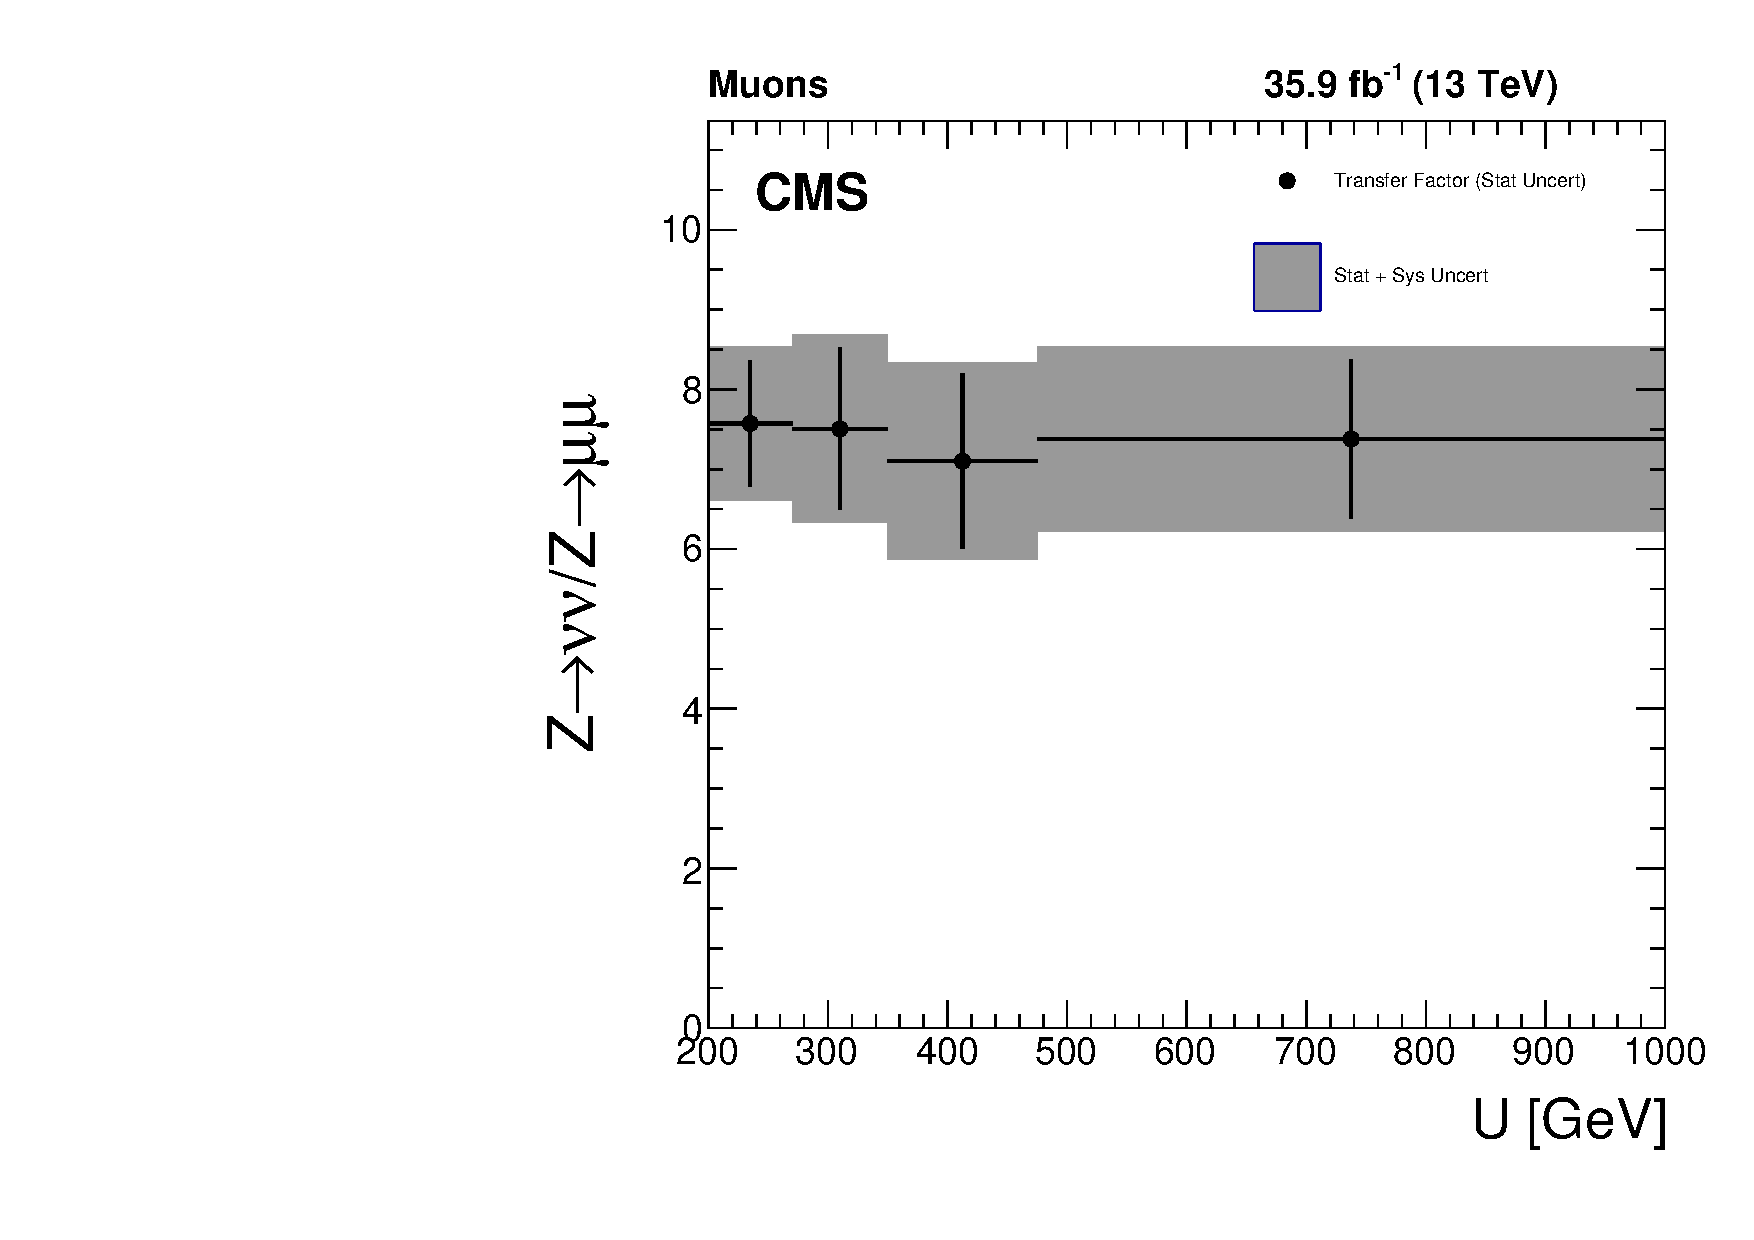
\includegraphics[width=0.3\textwidth]{figures/limits/rfactor_dimuon.pdf}}
   \subfloat{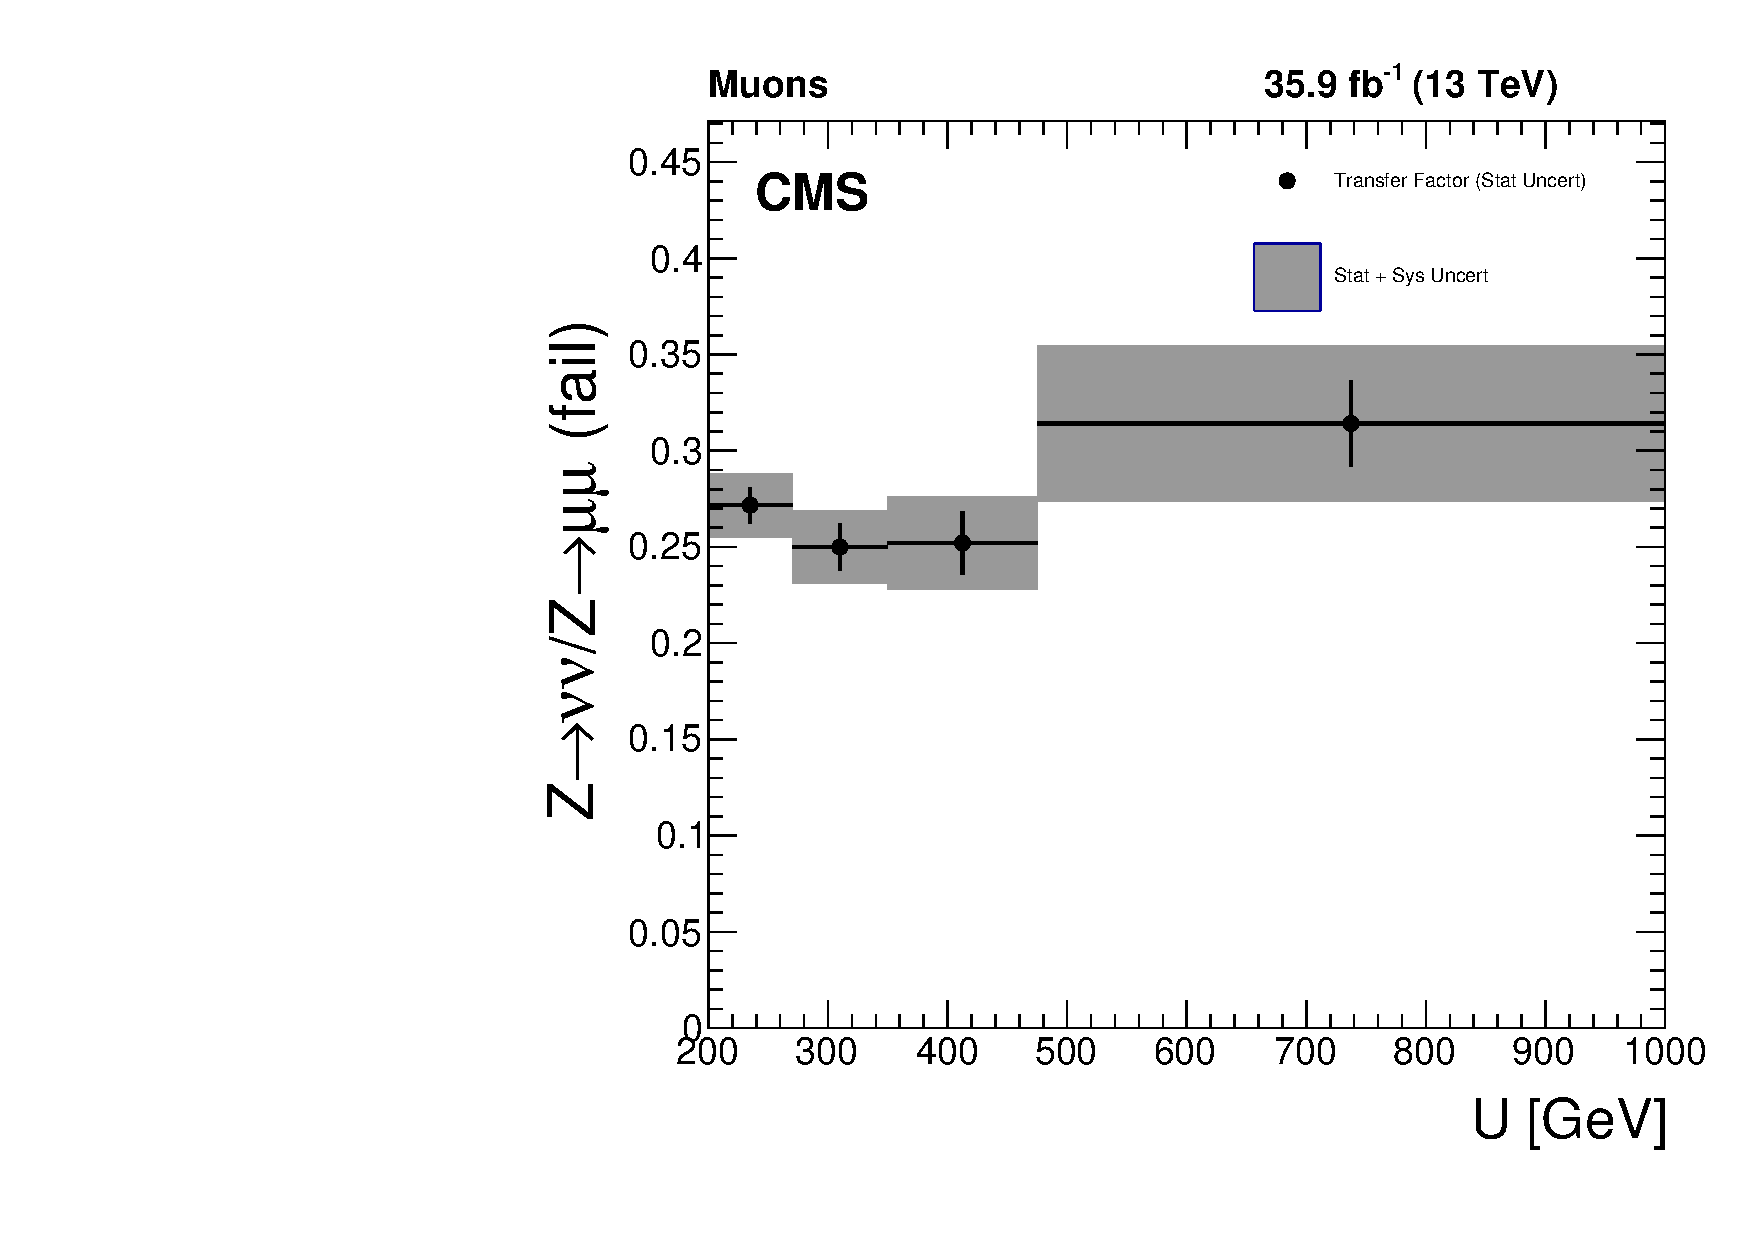
\includegraphics[width=0.3\textwidth]{figures/limits/rfactor_dimuon_fail.pdf}} \\
   \subfloat{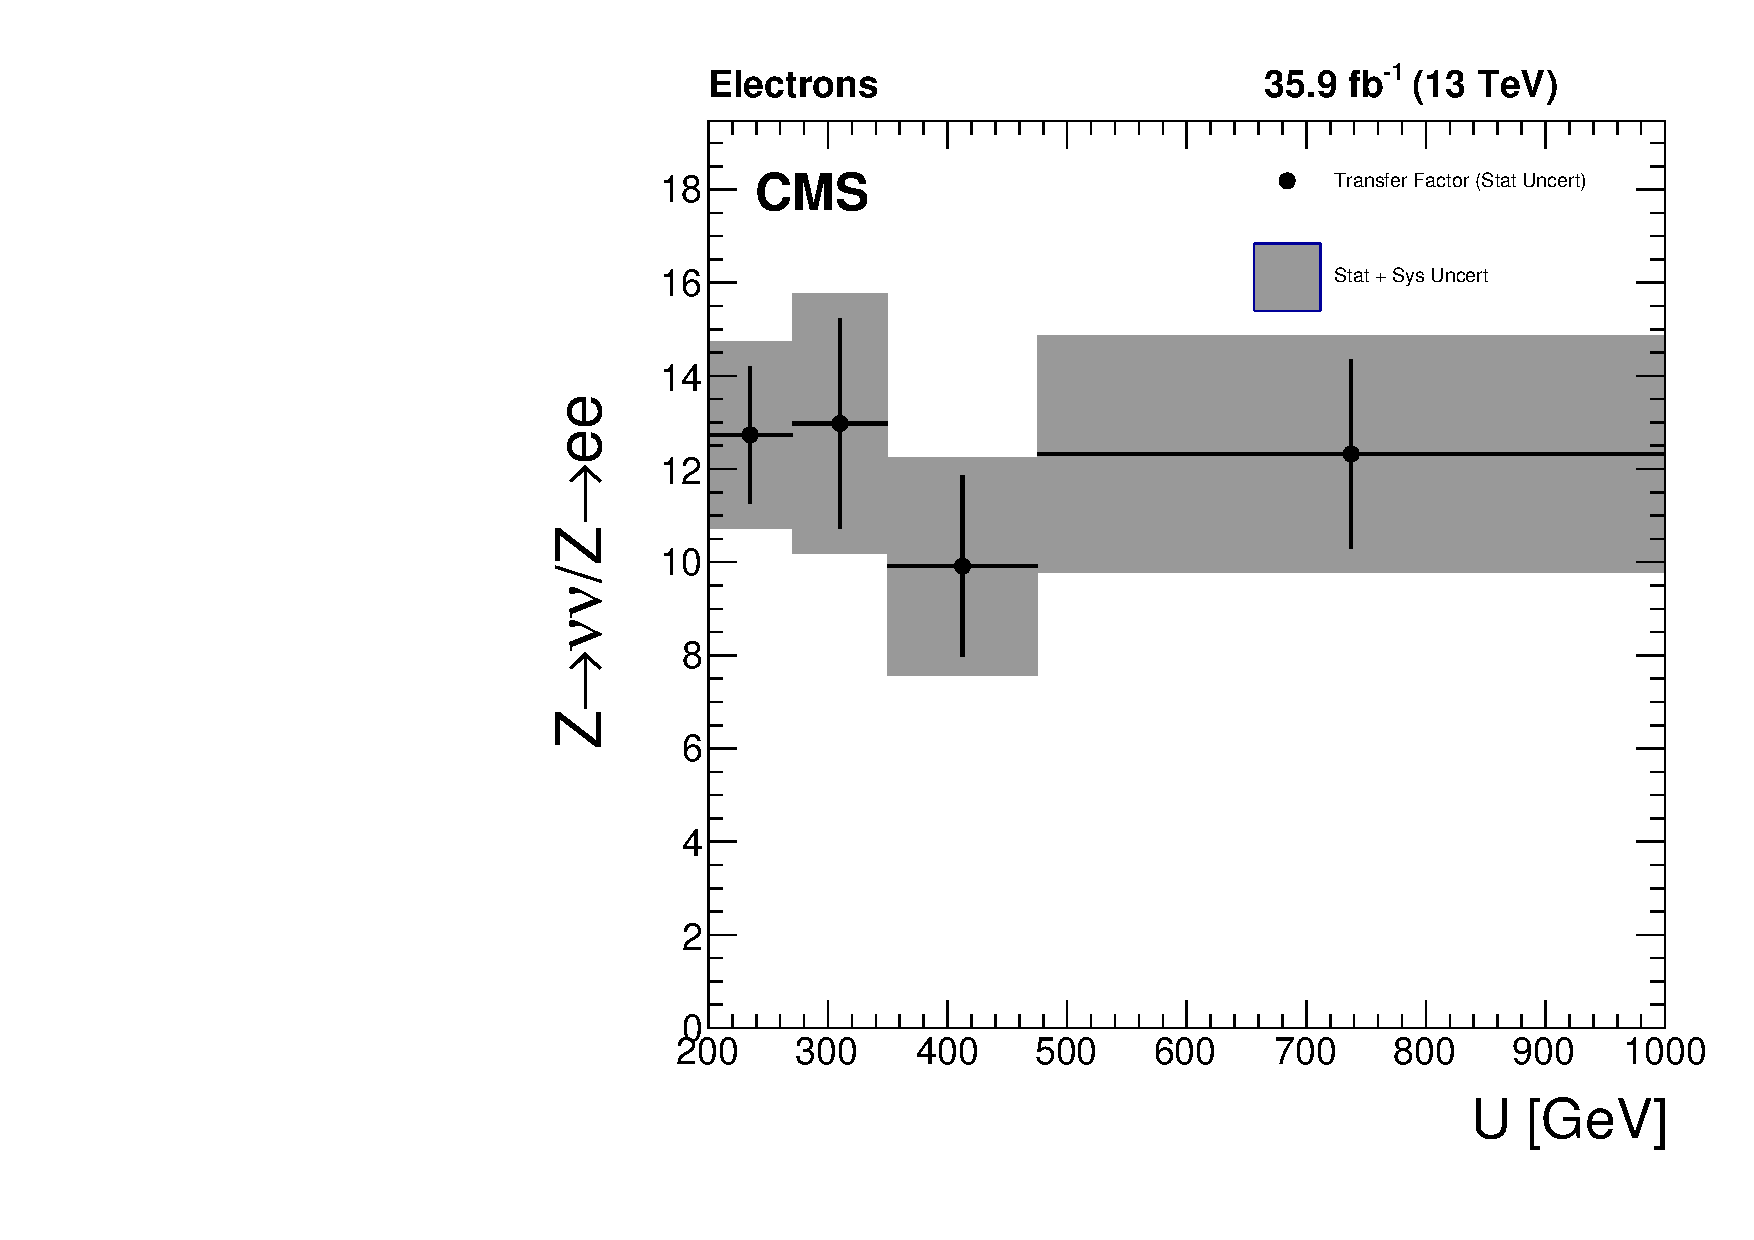
\includegraphics[width=0.3\textwidth]{figures/limits/rfactor_dielectron.pdf}}
   \subfloat{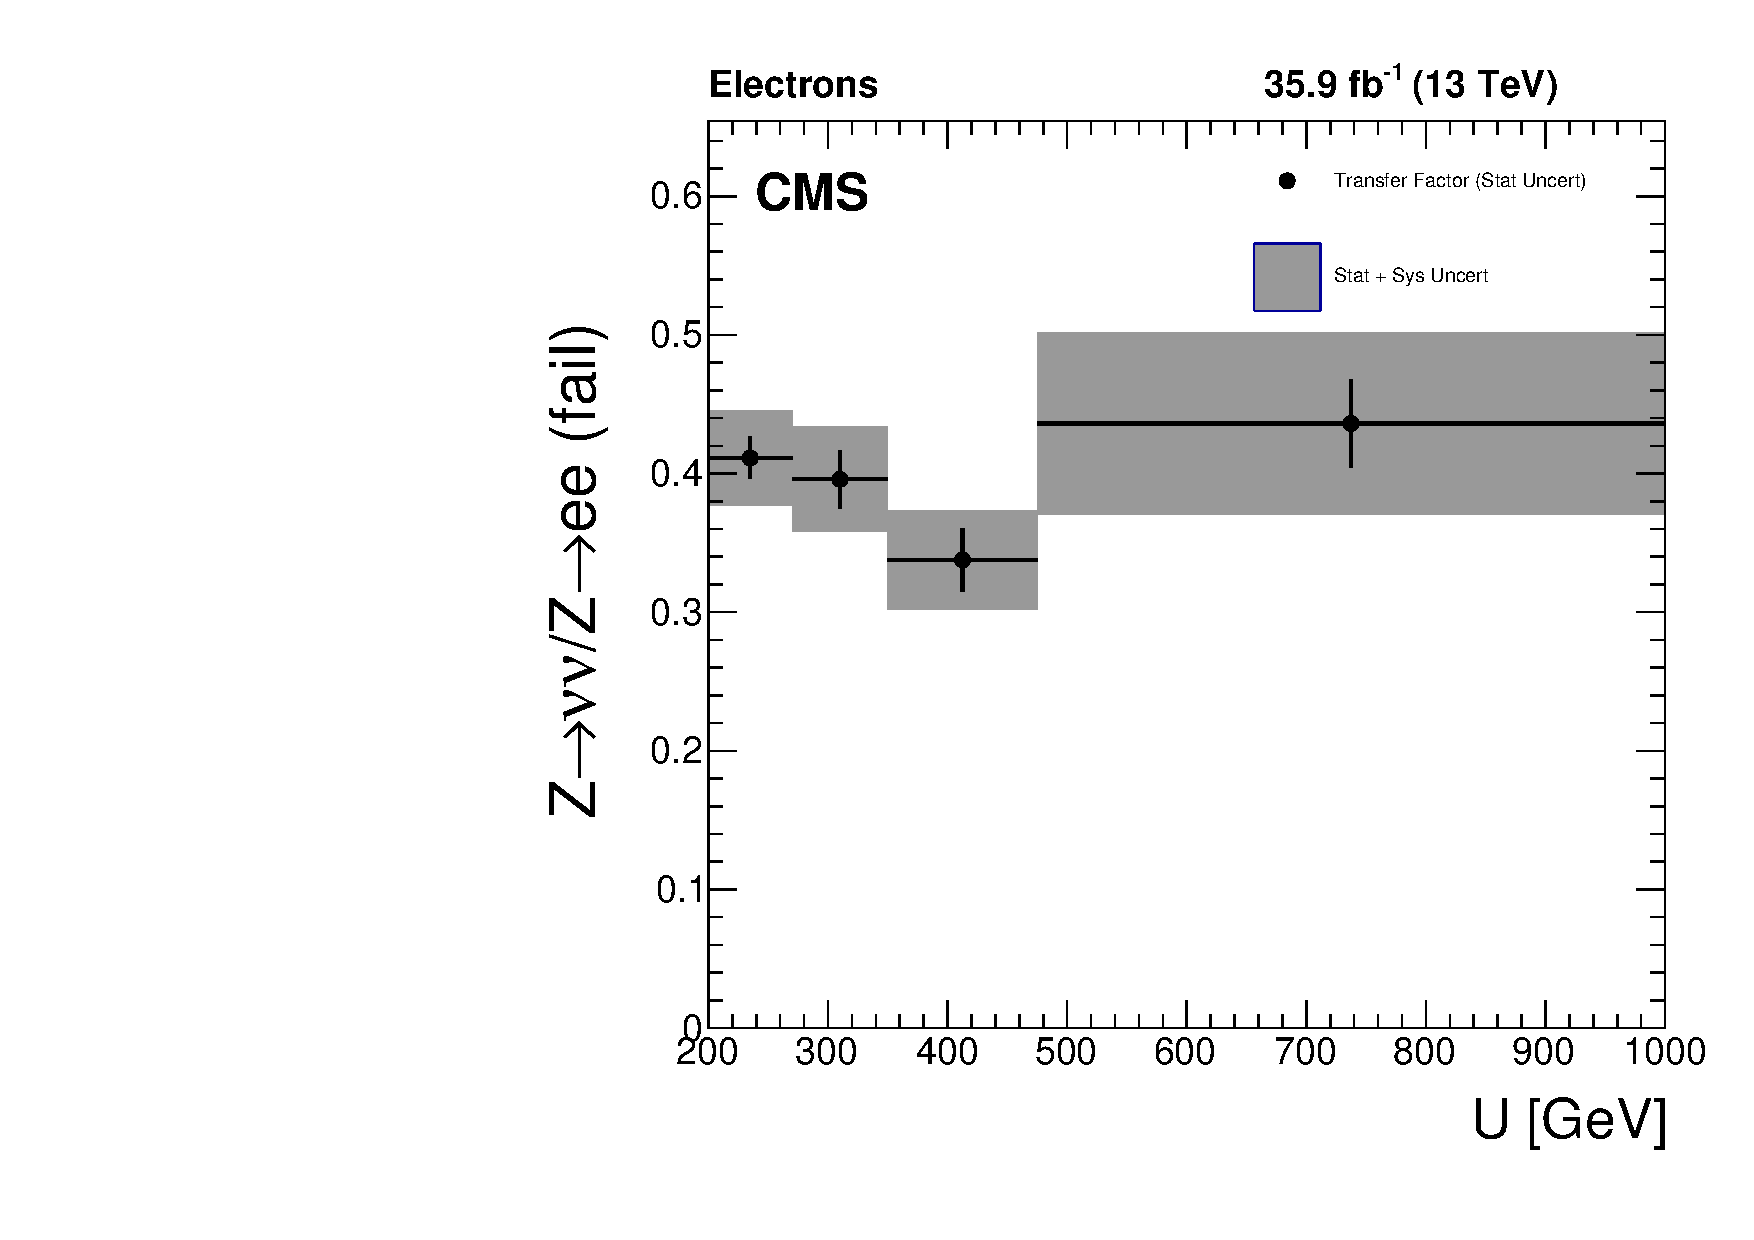
\includegraphics[width=0.3\textwidth]{figures/limits/rfactor_dielectron_fail.pdf}} \\
   \caption{Transfer factors to estimate $Z\rightarrow\nu\nu$ in the signal regions}
  \label{fig:xferZvv}
\end{figure}


\begin{figure}[htbp]
  \centering
  \subfigure[$t\bar{t}$ in $t\bar{t}$ pass CR]{
    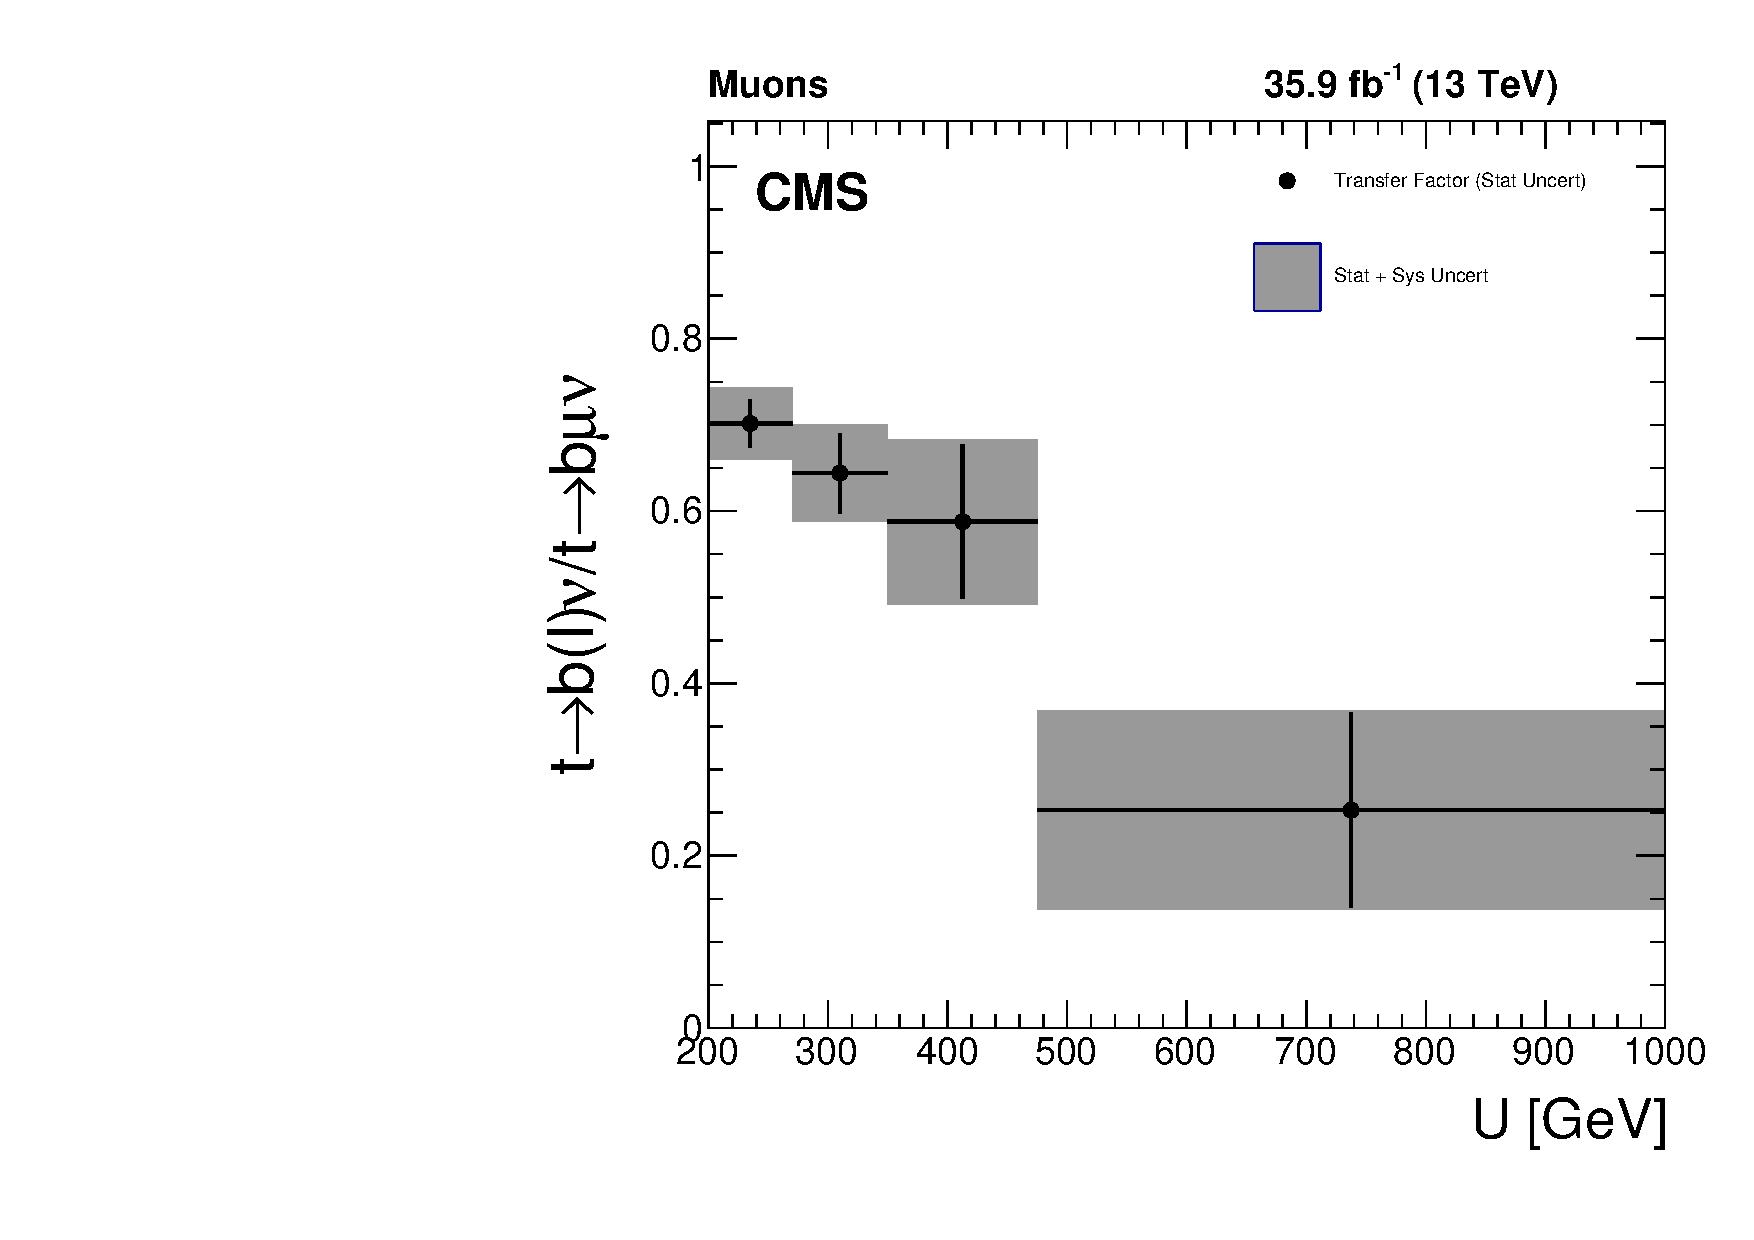
\includegraphics[width=0.25\textwidth]{figures/limits/rfactor_singlemuontop.pdf}
    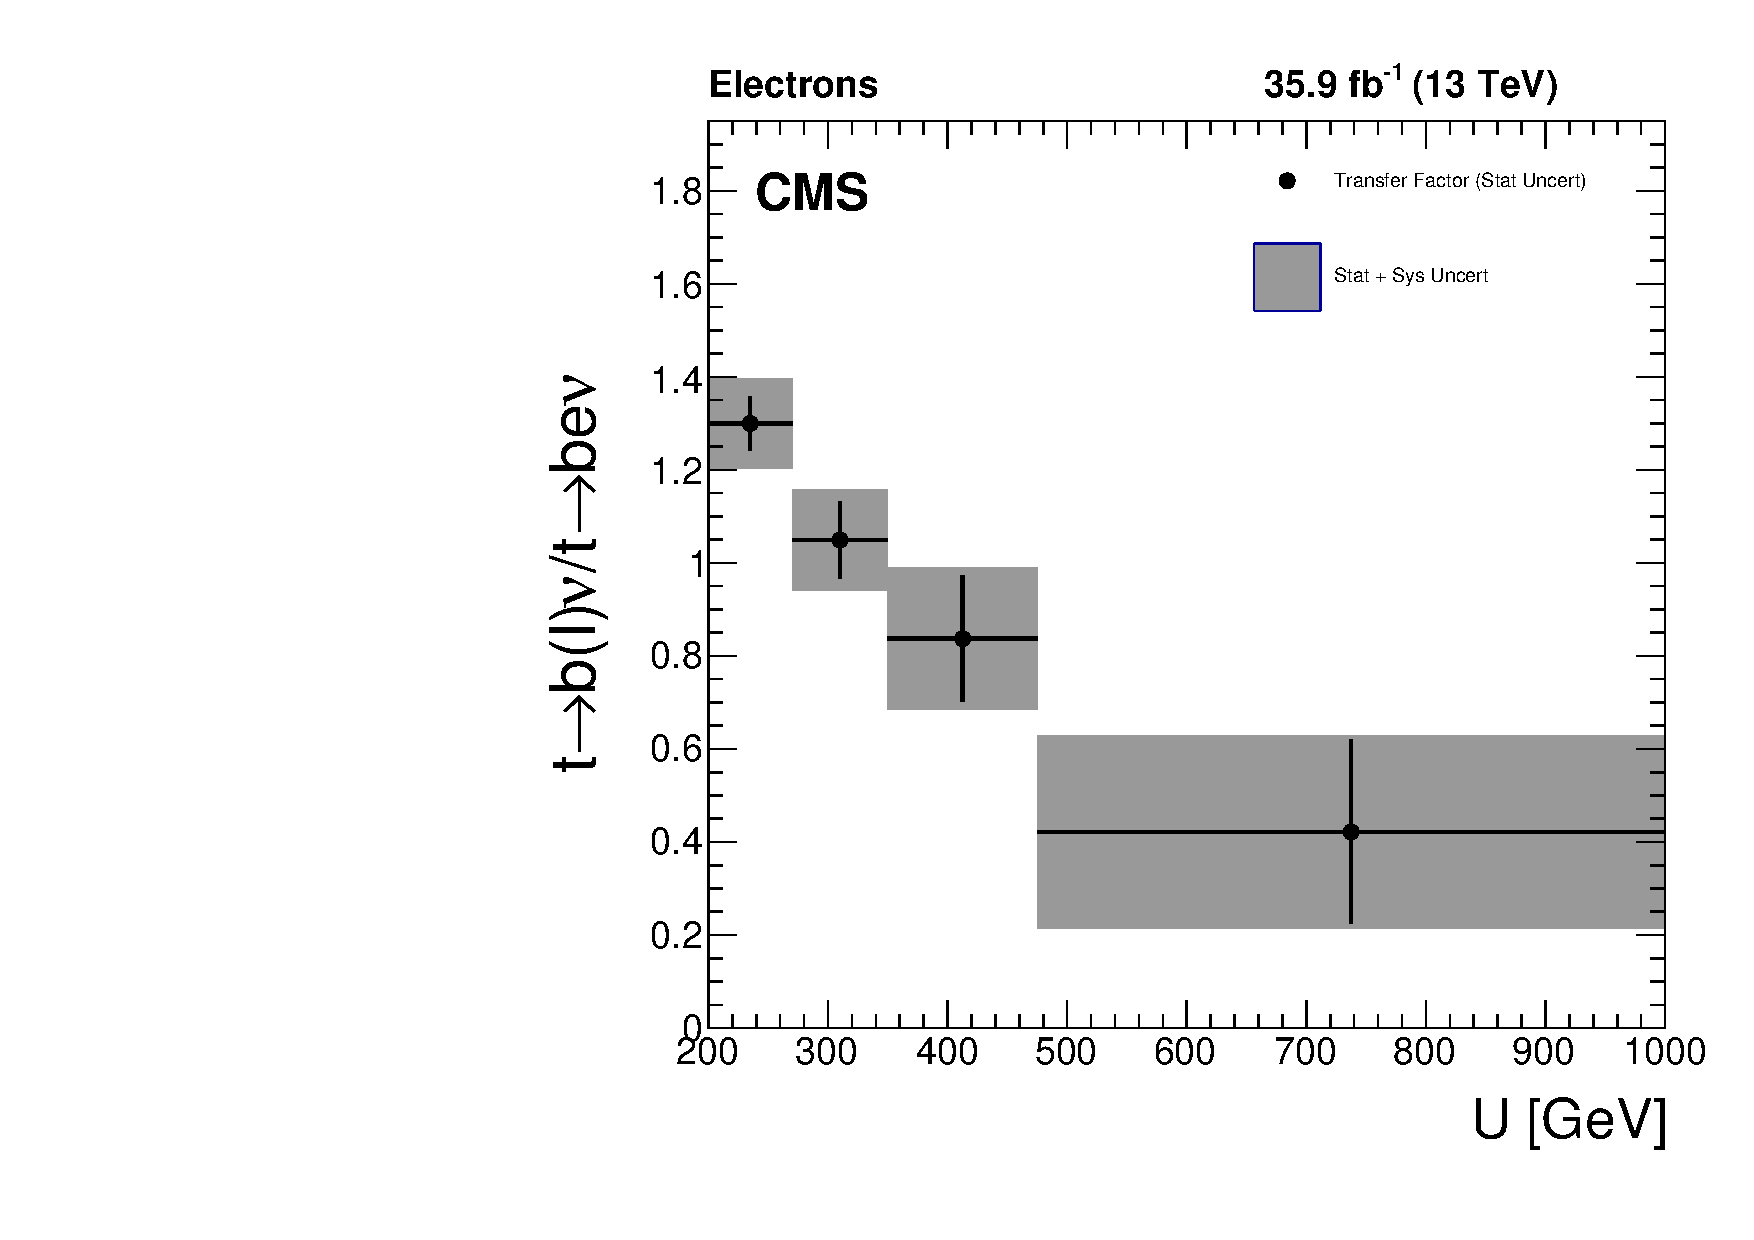
\includegraphics[width=0.25\textwidth]{figures/limits/rfactor_singleelectrontop.pdf}
  }
  \subfigure[$t\bar{t}$ in $W$ pass CR]{
    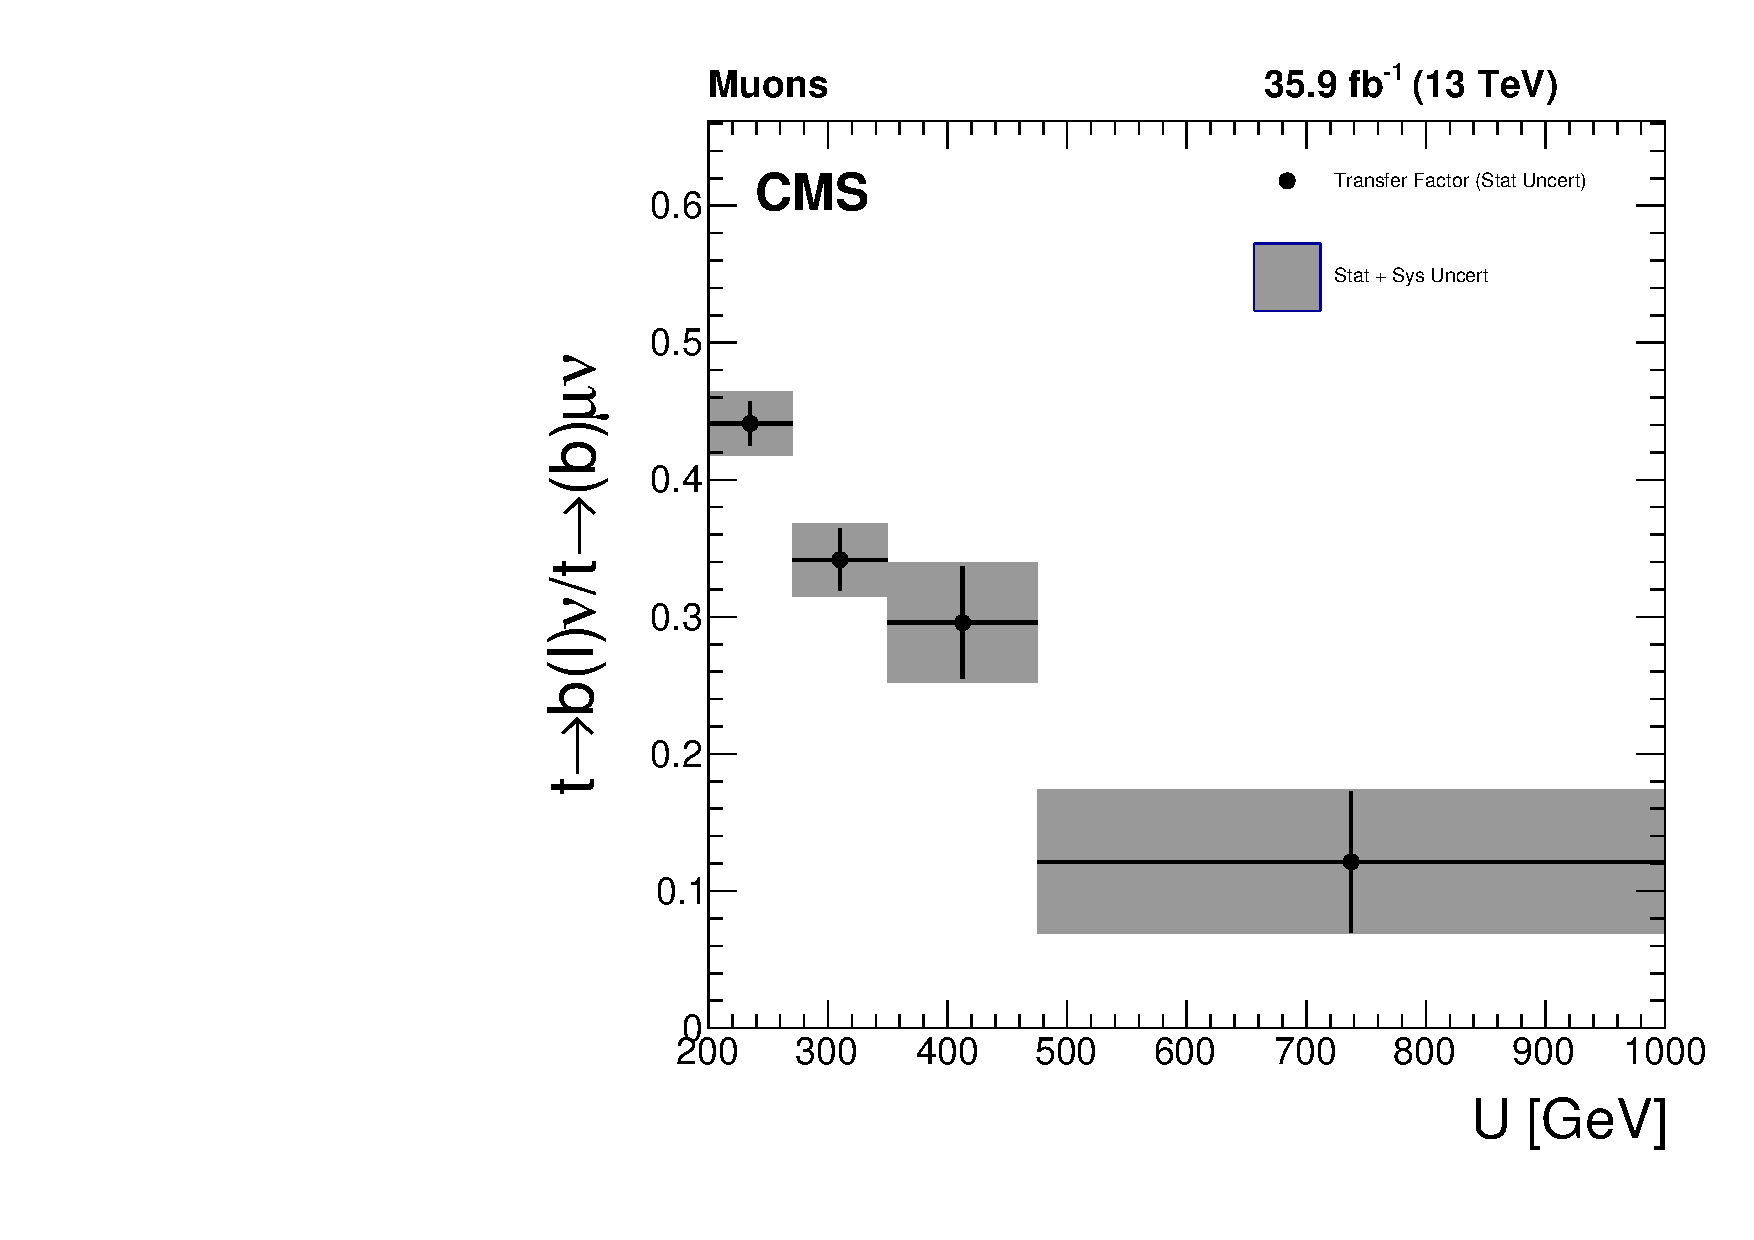
\includegraphics[width=0.25\textwidth]{figures/limits/rfactor_singlemuonwtop.pdf}
    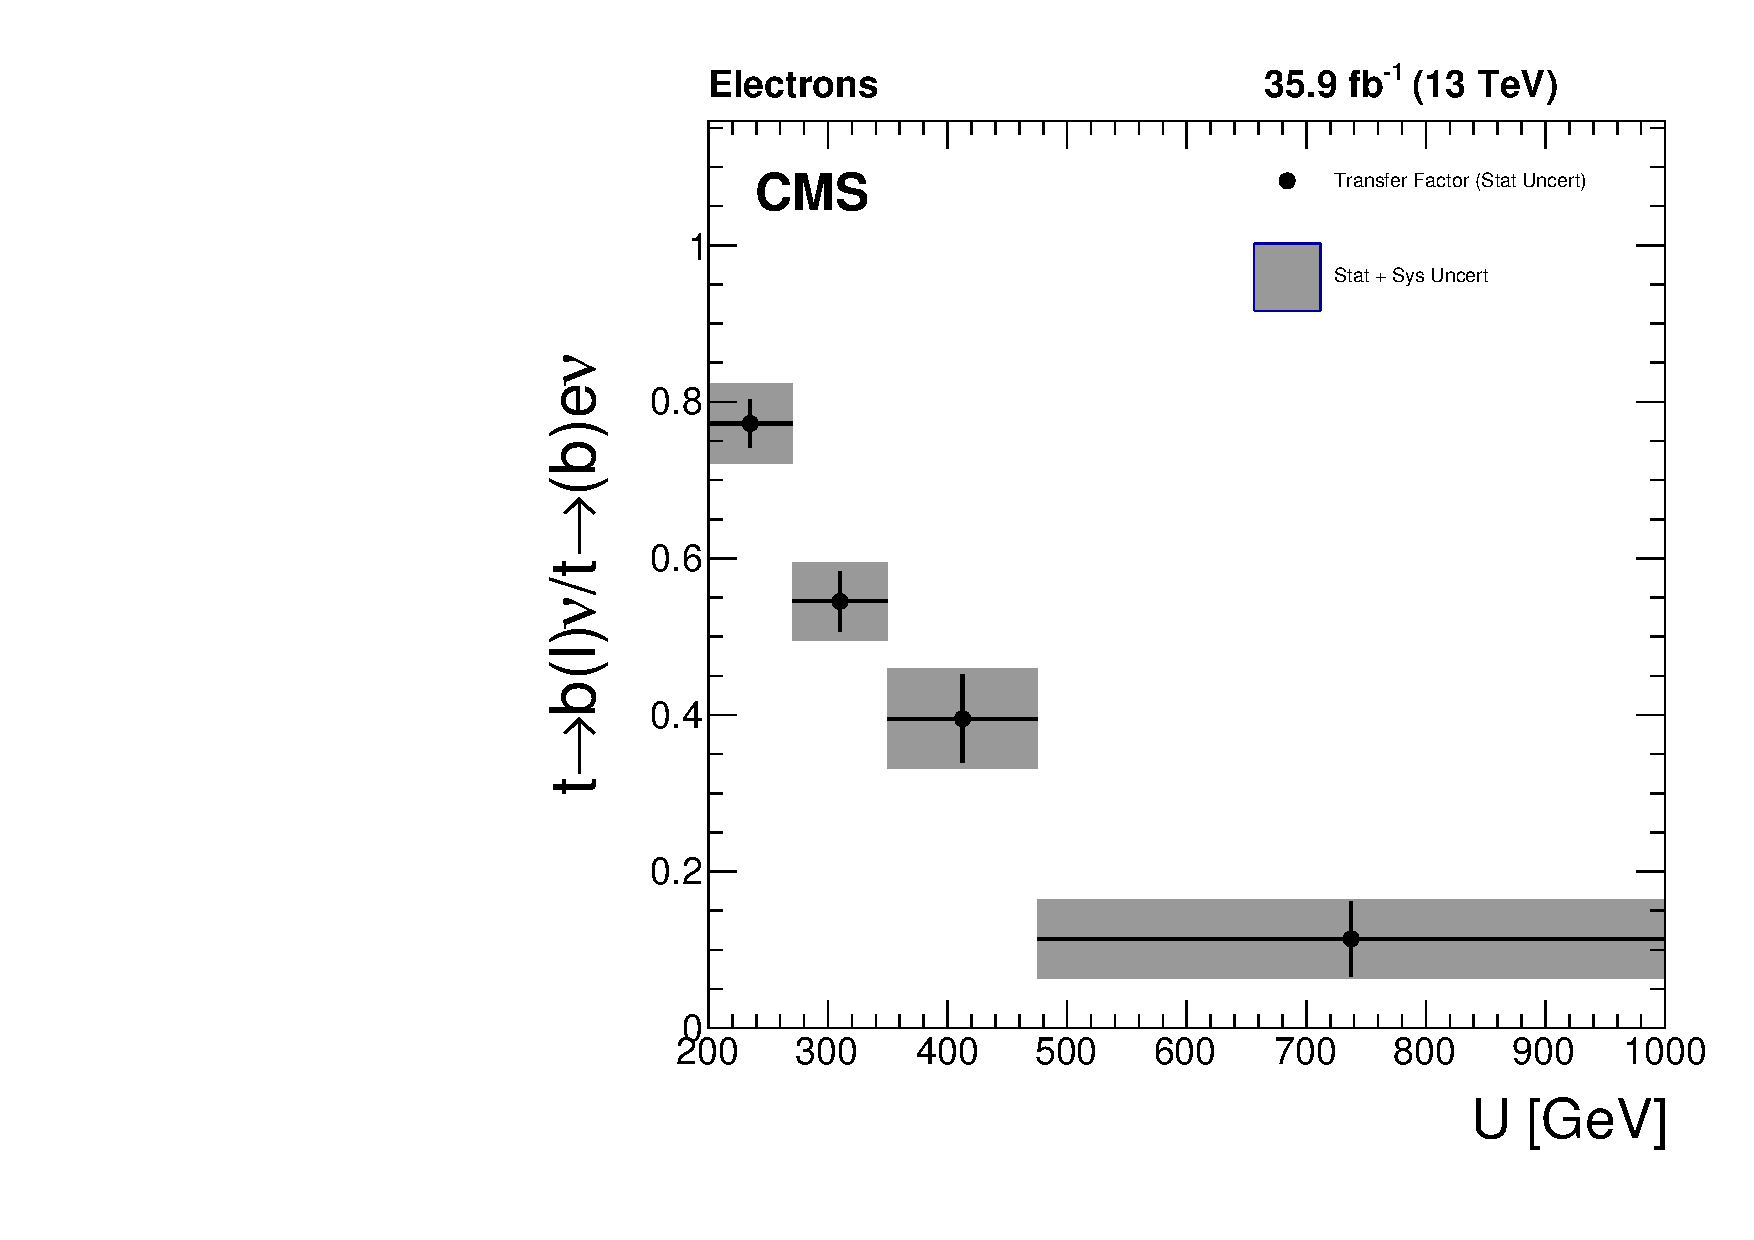
\includegraphics[width=0.25\textwidth]{figures/limits/rfactor_singleelectronwtop.pdf}
  }\\
  \subfigure[$t\bar{t}$ in $t\bar{t}$ fail CR]{
    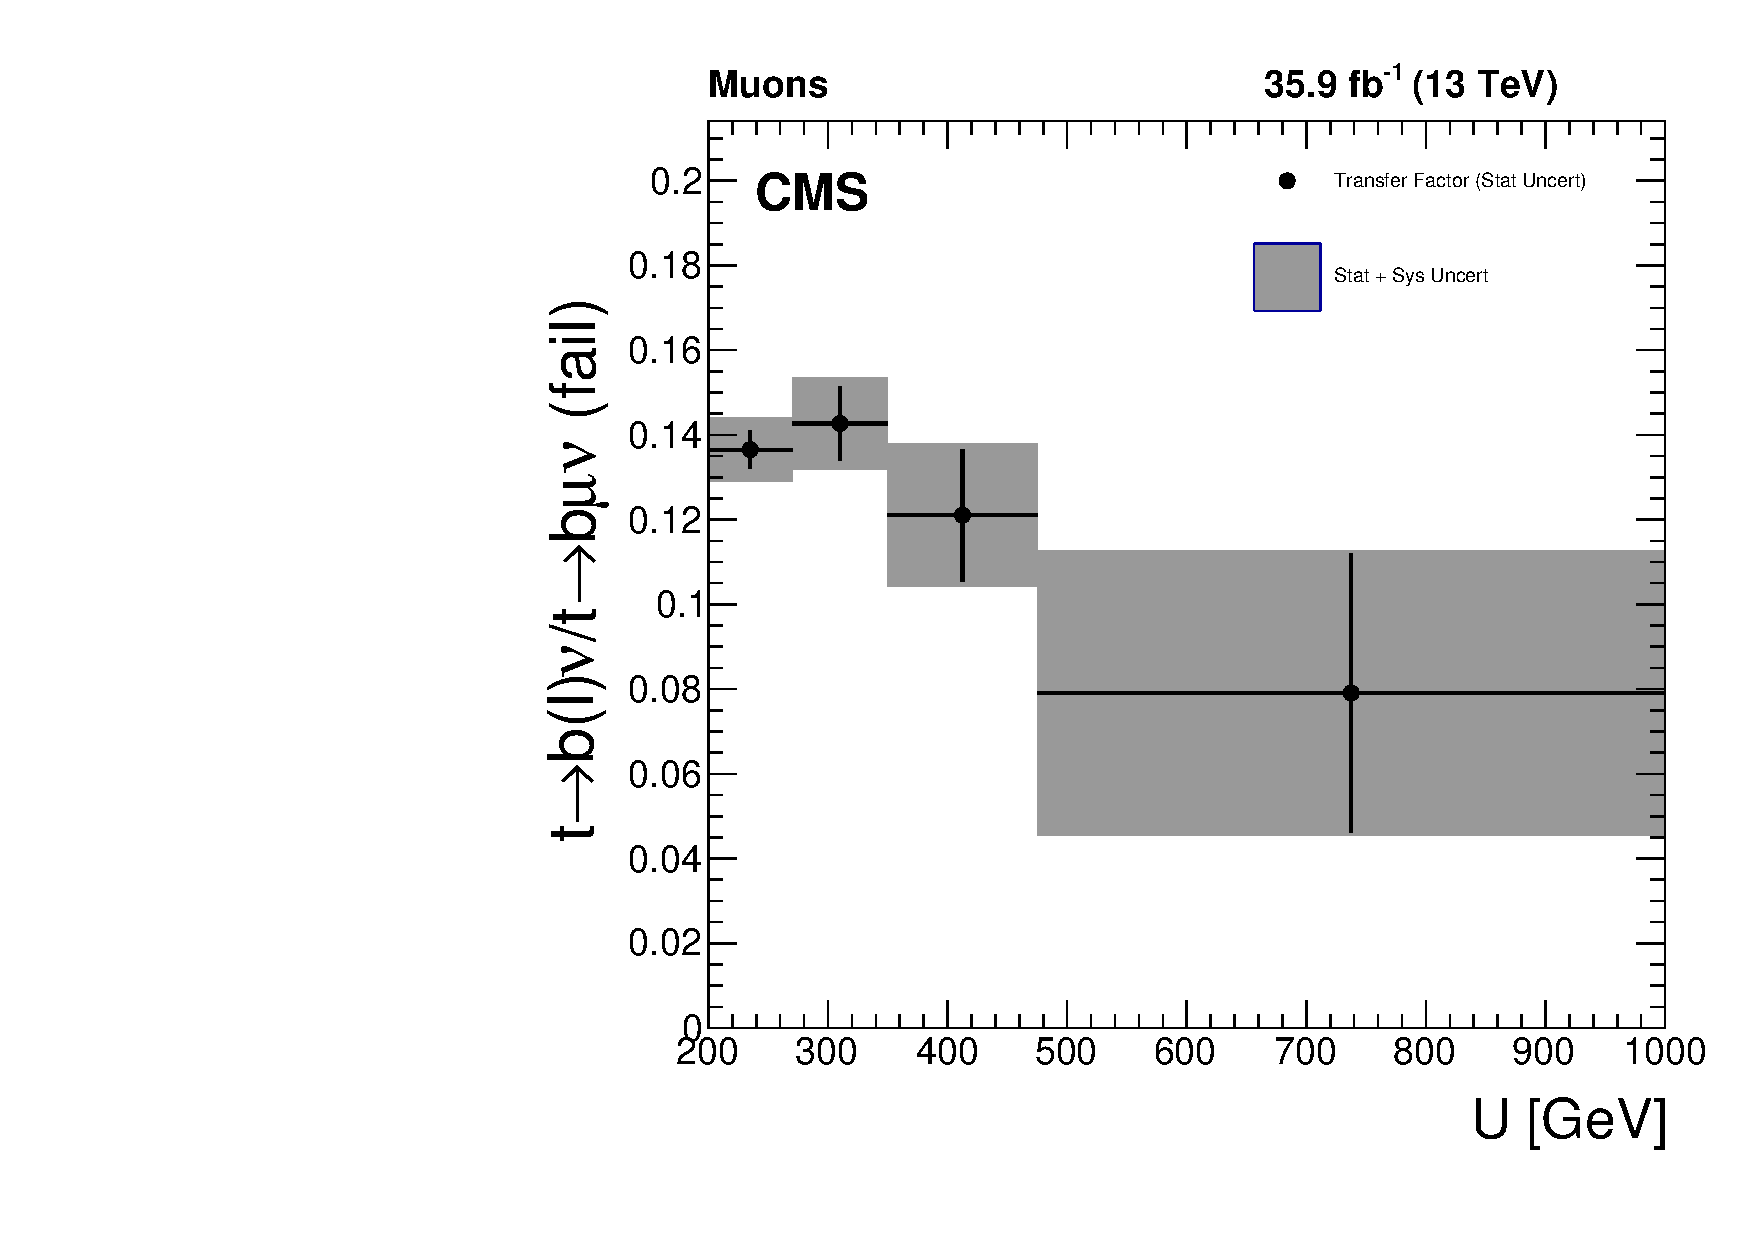
\includegraphics[width=0.25\textwidth]{figures/limits/rfactor_singlemuontop_fail.pdf}
    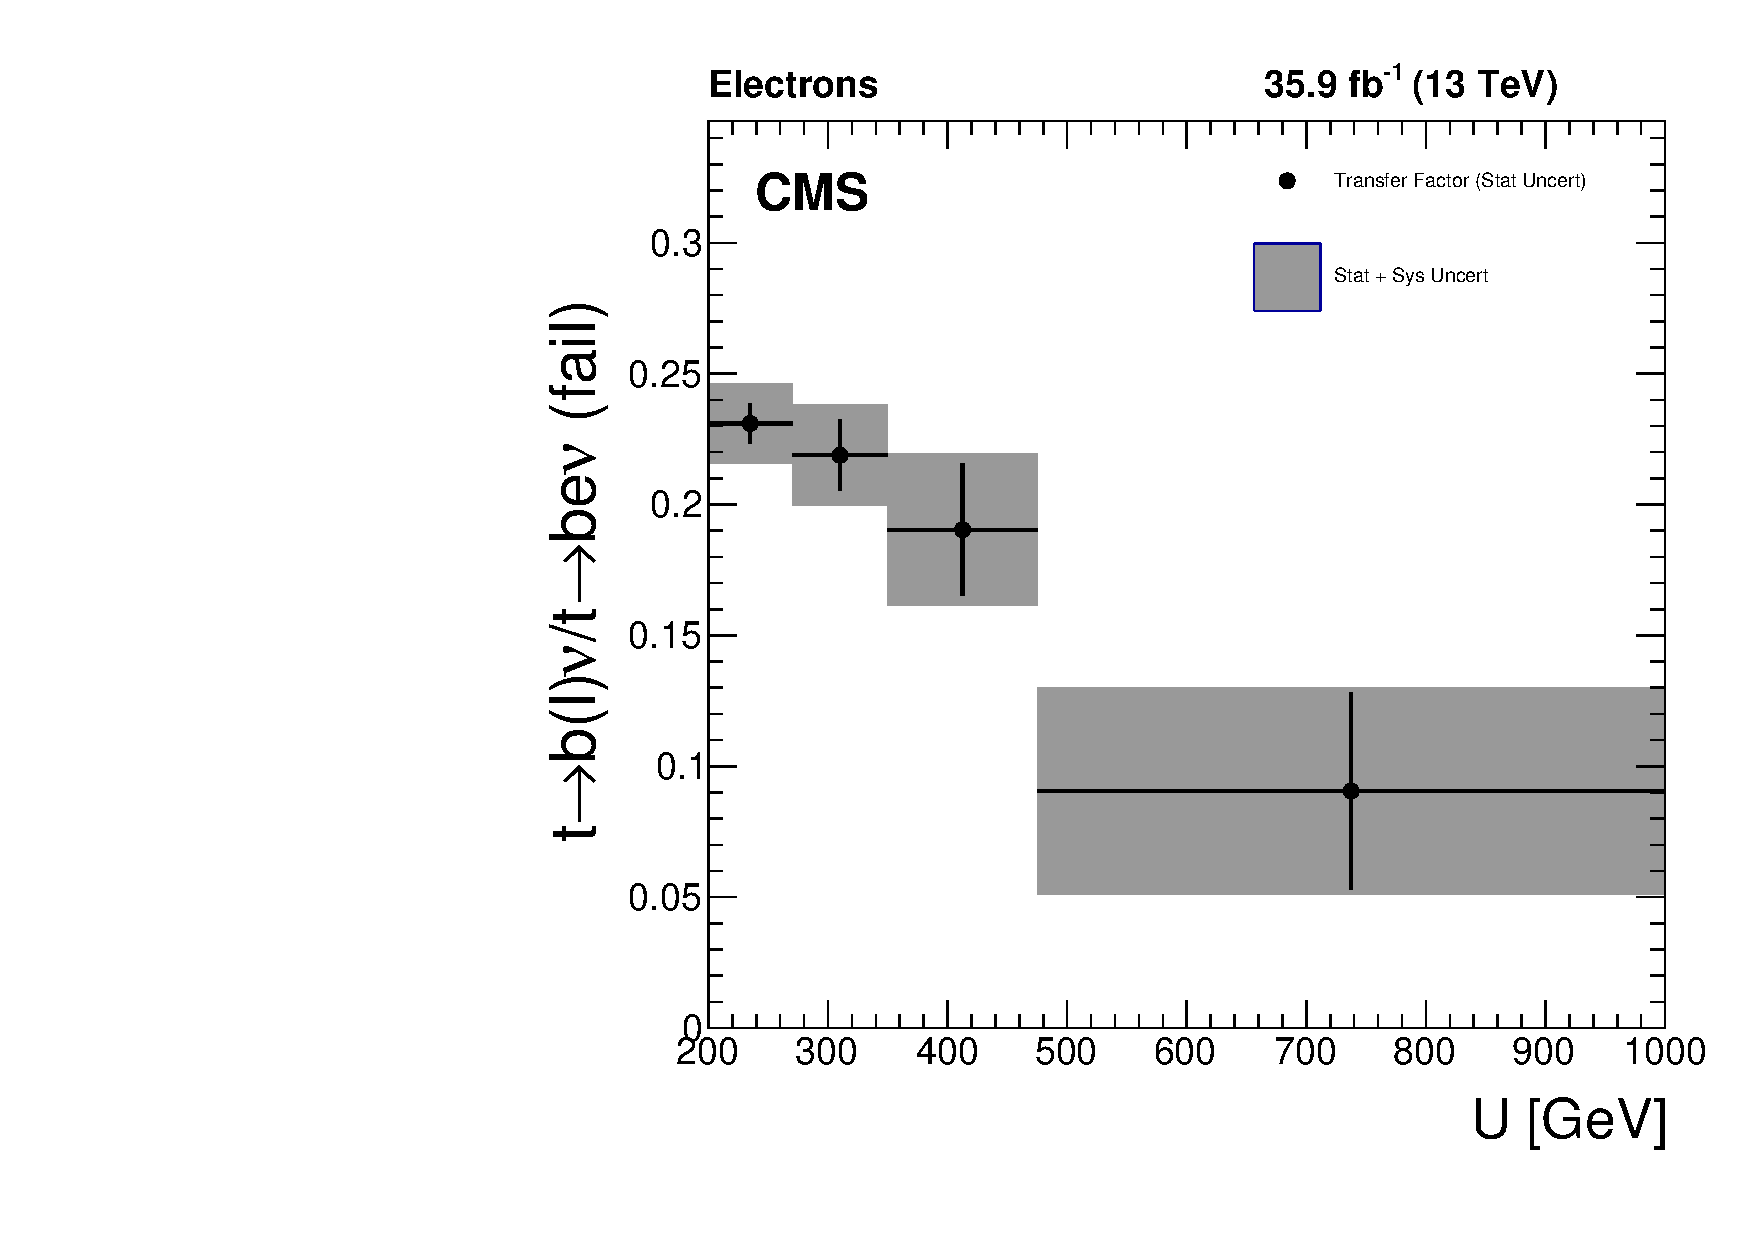
\includegraphics[width=0.25\textwidth]{figures/limits/rfactor_singleelectrontop_fail.pdf}
  }\\
  \caption{Transfer factors that link $t\bar{t}$ in the signal region to $t\bar{t}$ in the control regions}
  \label{fig:xferTT}
\end{figure}


\begin{figure}[htbp]
  \centering
  \subfigure[$W$+jets in $W$+jets pass CR]{
    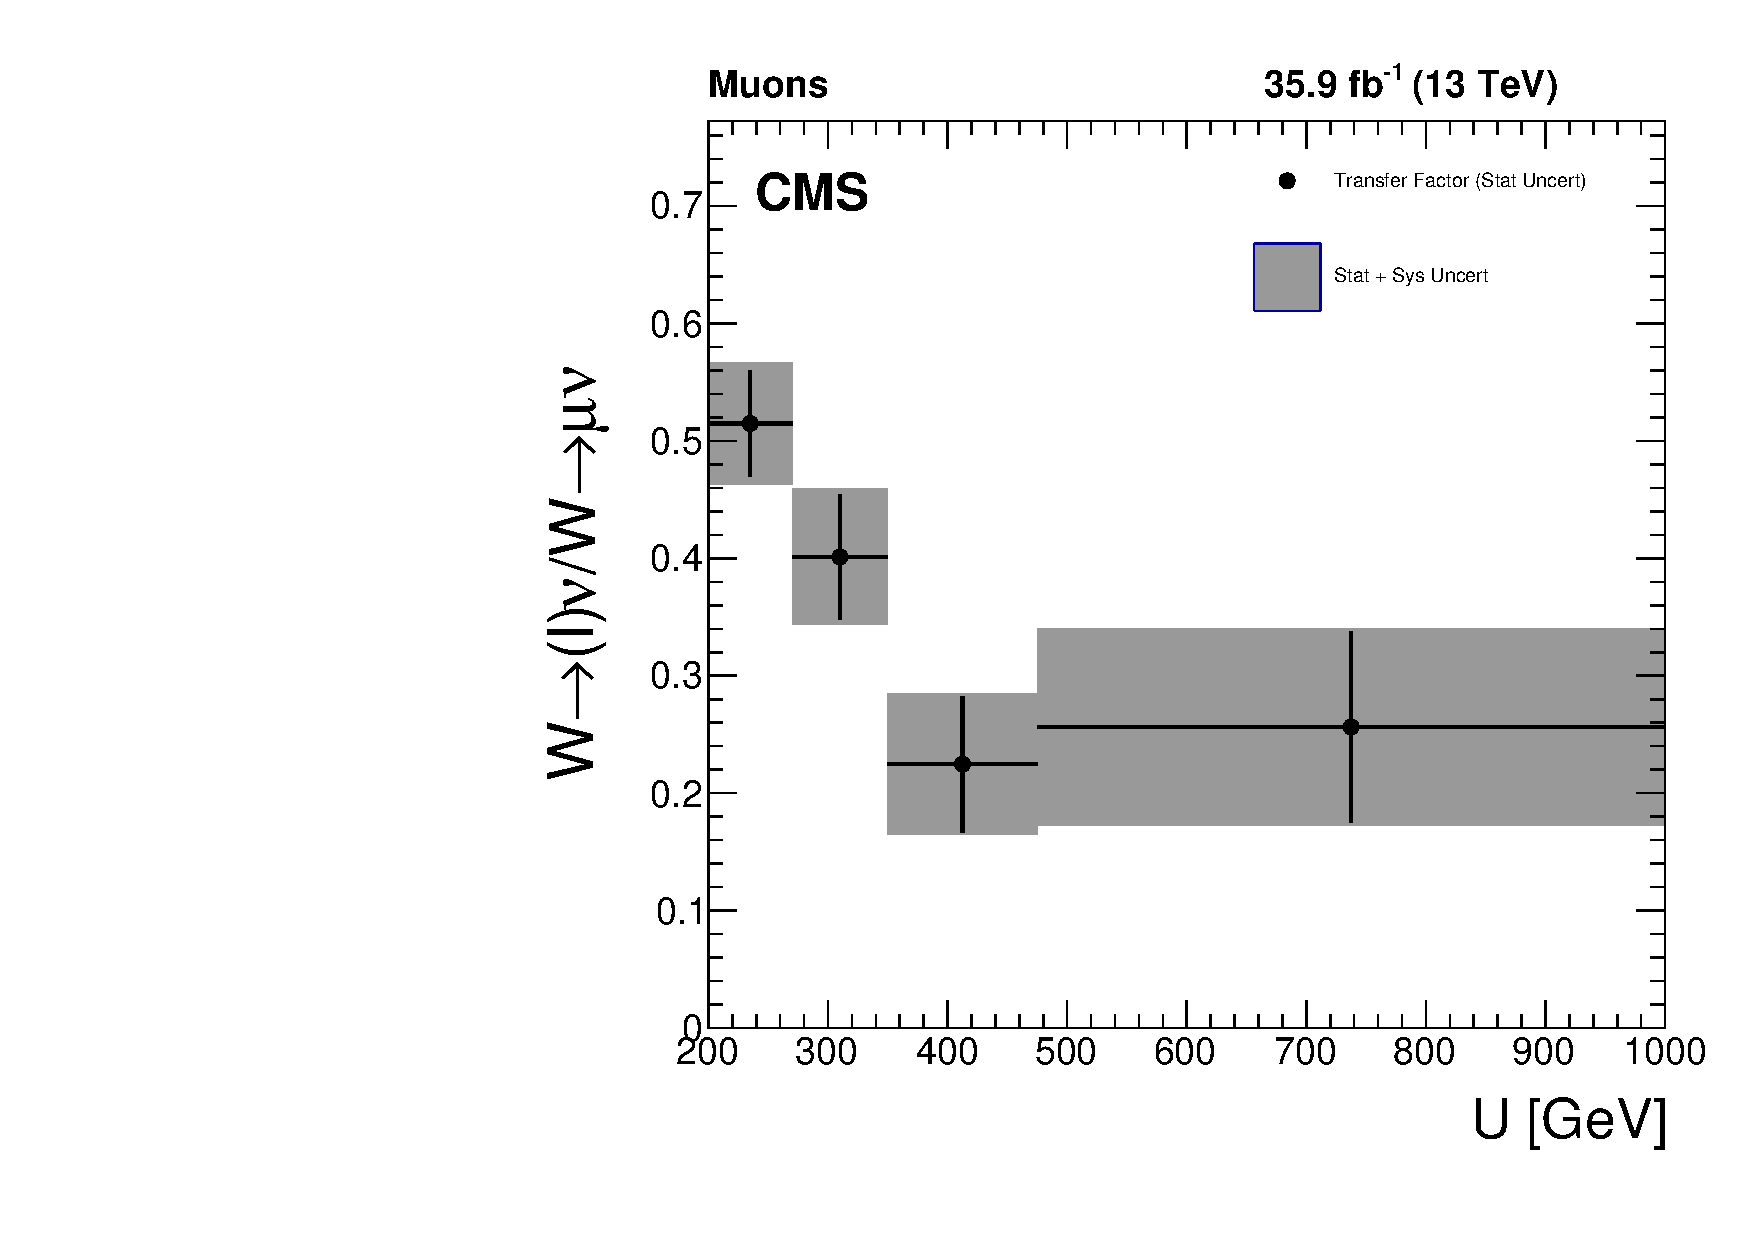
\includegraphics[width=0.25\textwidth]{figures/limits/rfactor_singlemuonw.pdf}
    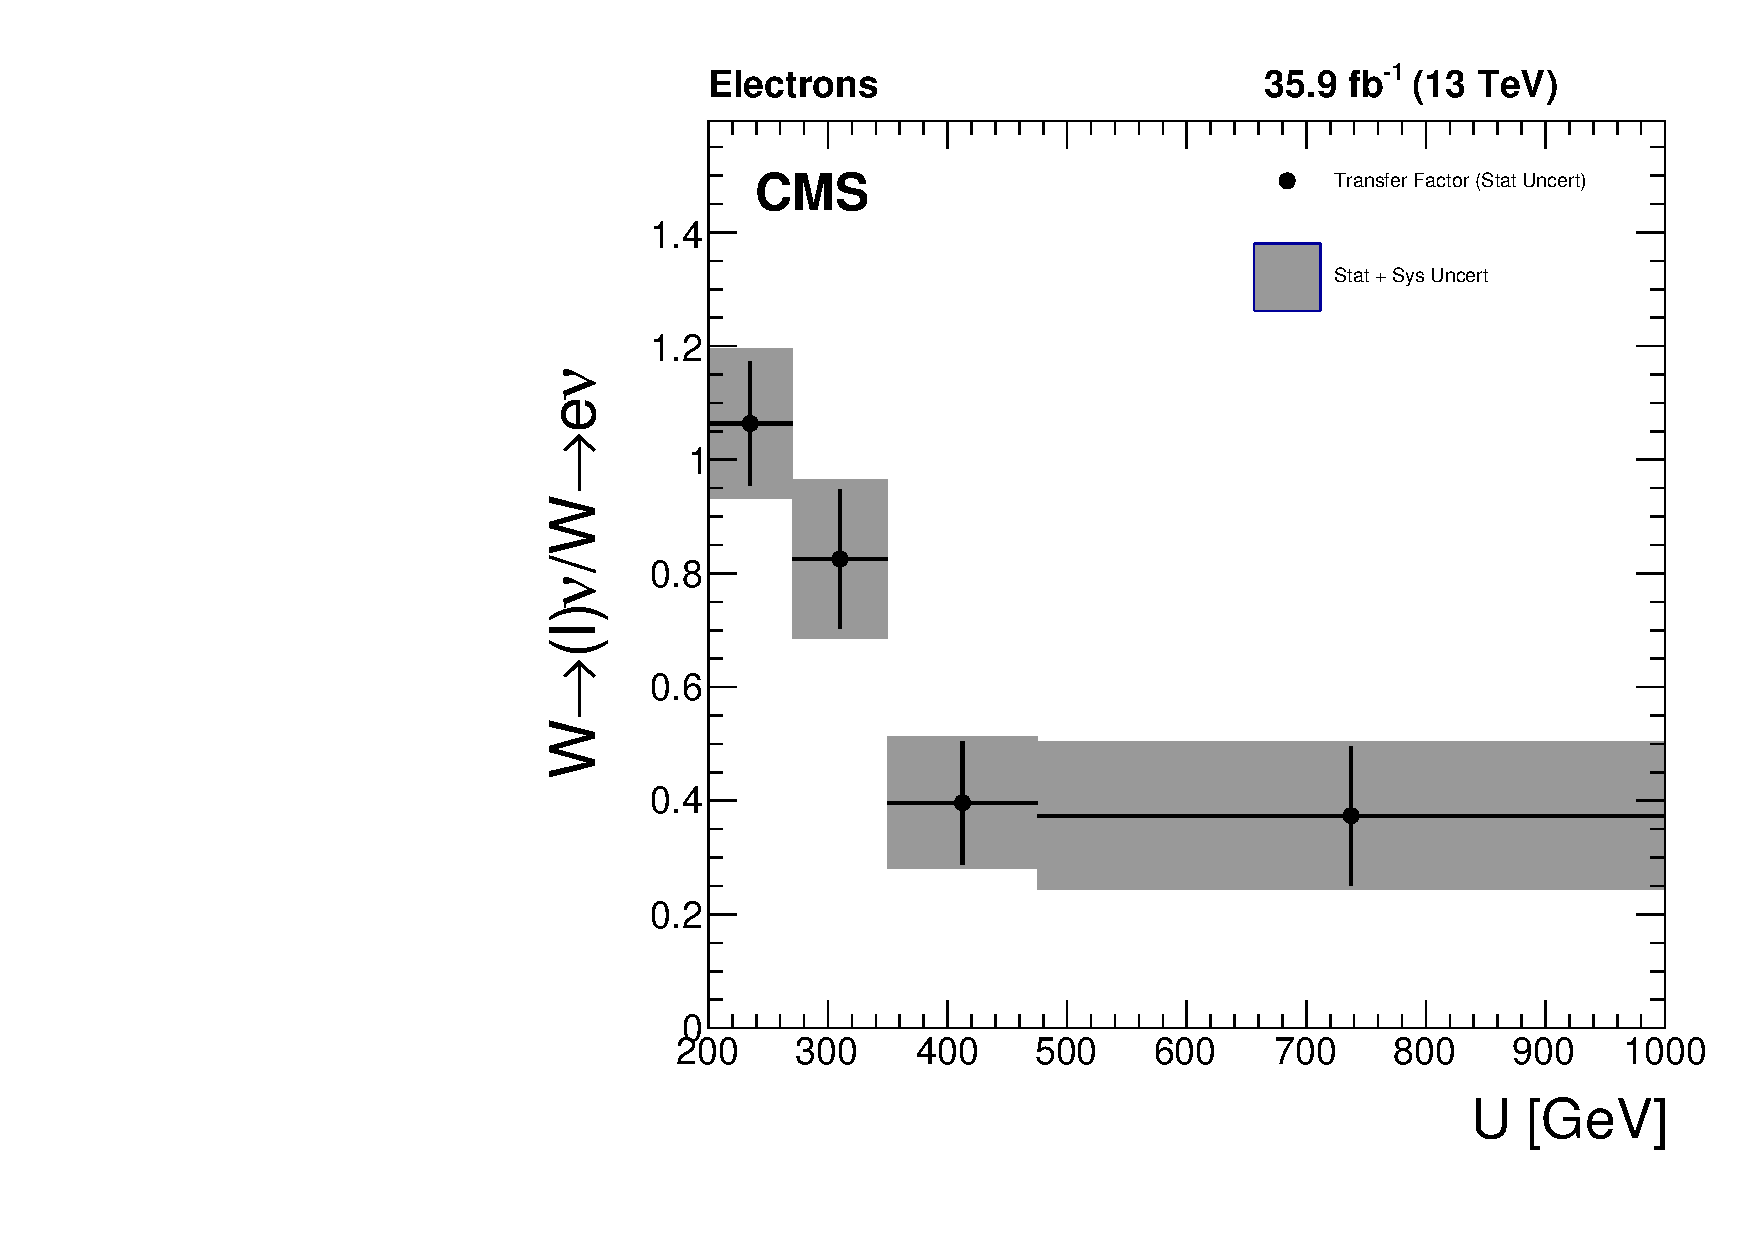
\includegraphics[width=0.25\textwidth]{figures/limits/rfactor_singleelectronw.pdf}
  }
  \subfigure[$W$+jets in $W$ fail CR]{
    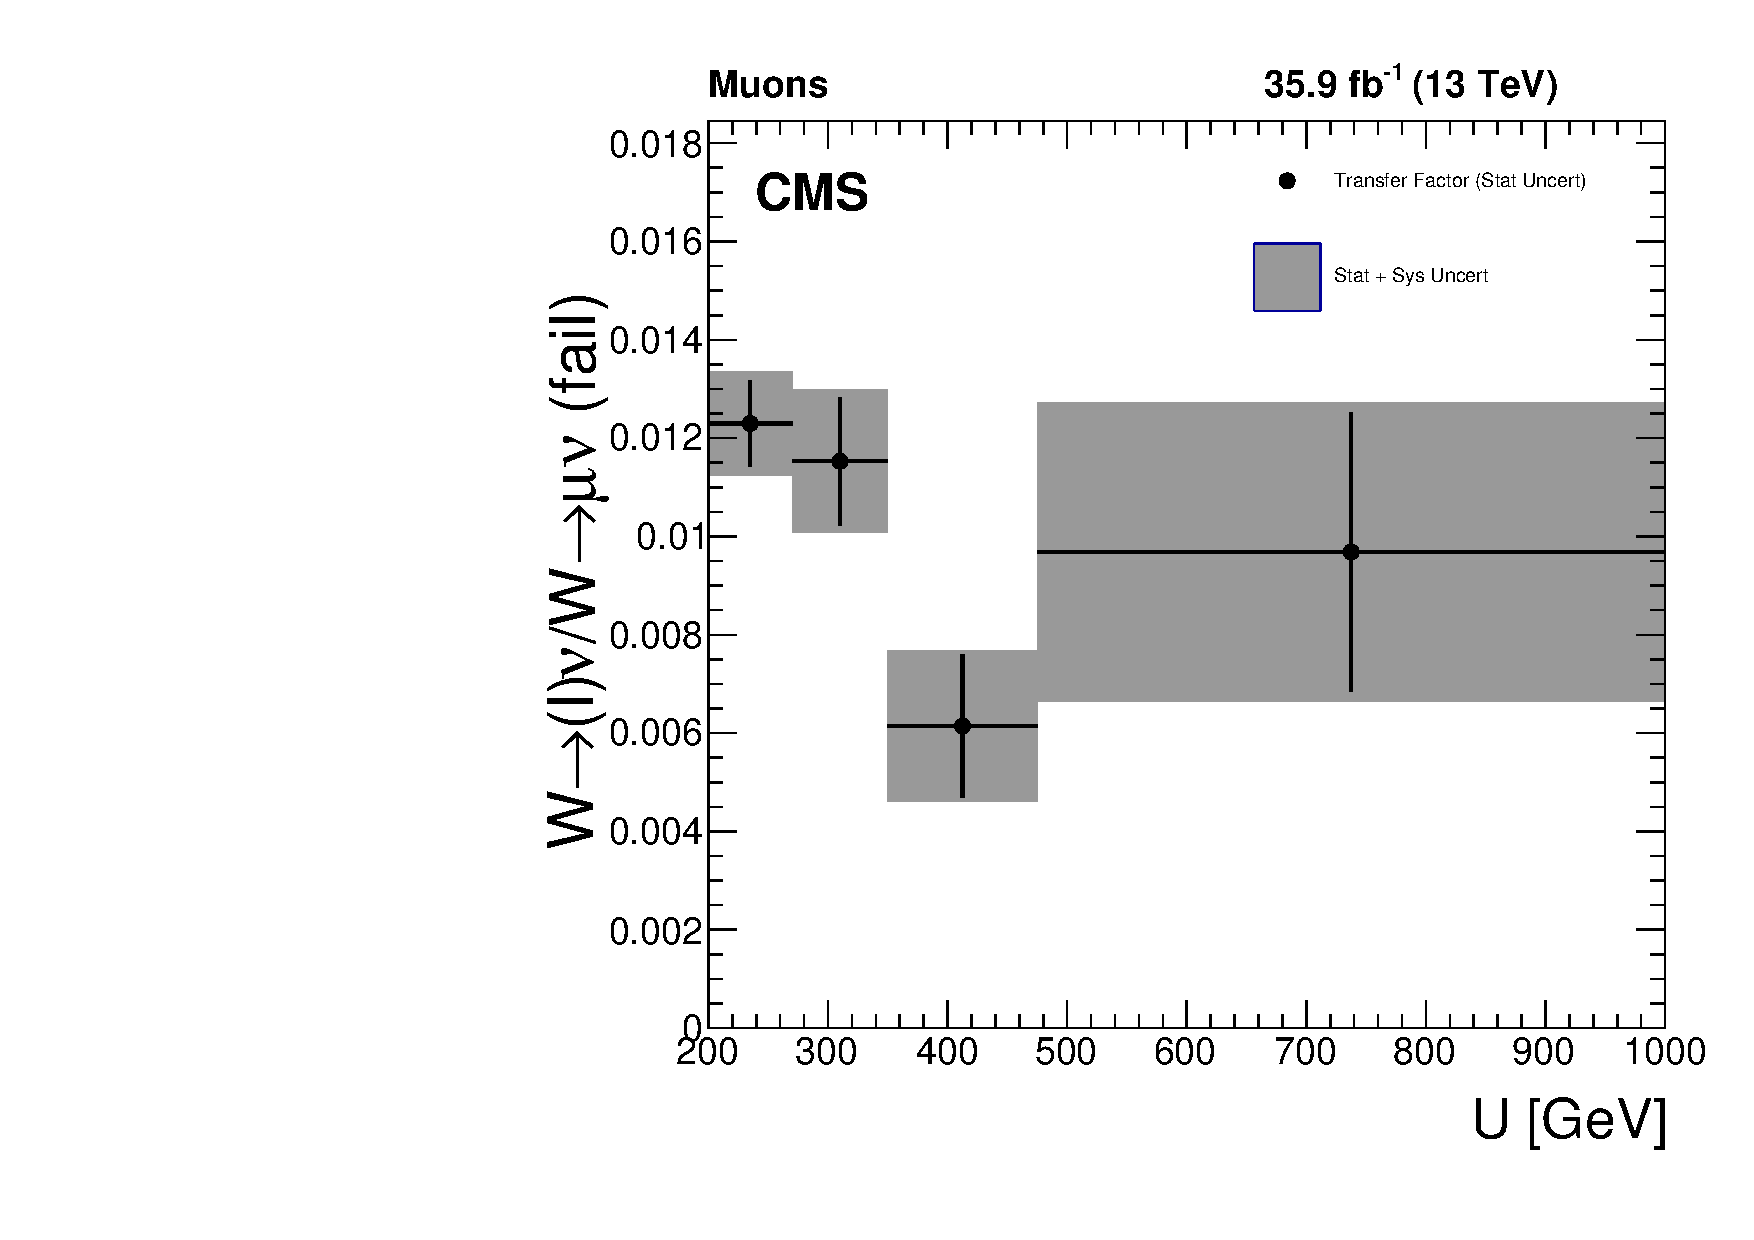
\includegraphics[width=0.25\textwidth]{figures/limits/rfactor_singlemuonw_fail.pdf}
    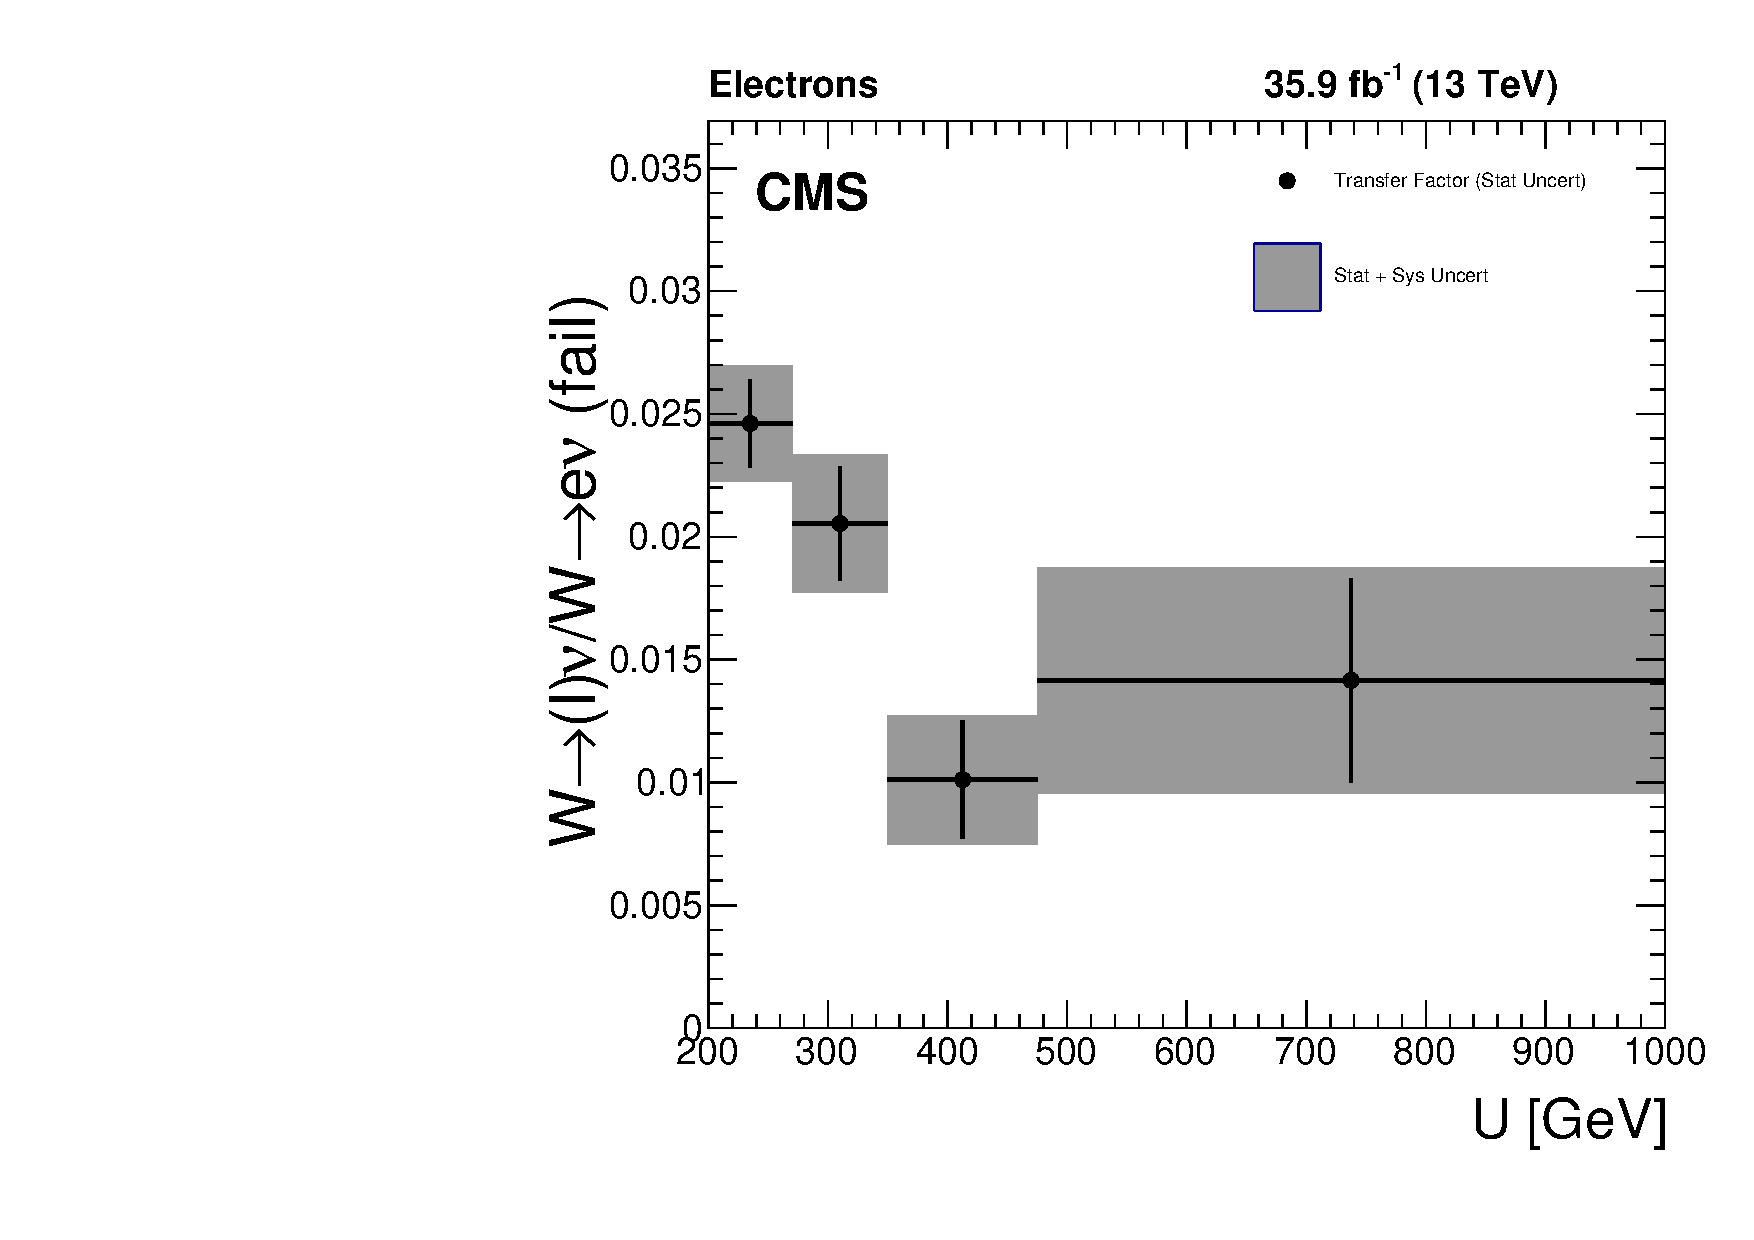
\includegraphics[width=0.25\textwidth]{figures/limits/rfactor_singleelectronw_fail.pdf}
  }\\
  \subfigure[$W$+jets in $t\bar{t}$ fail CR]{
    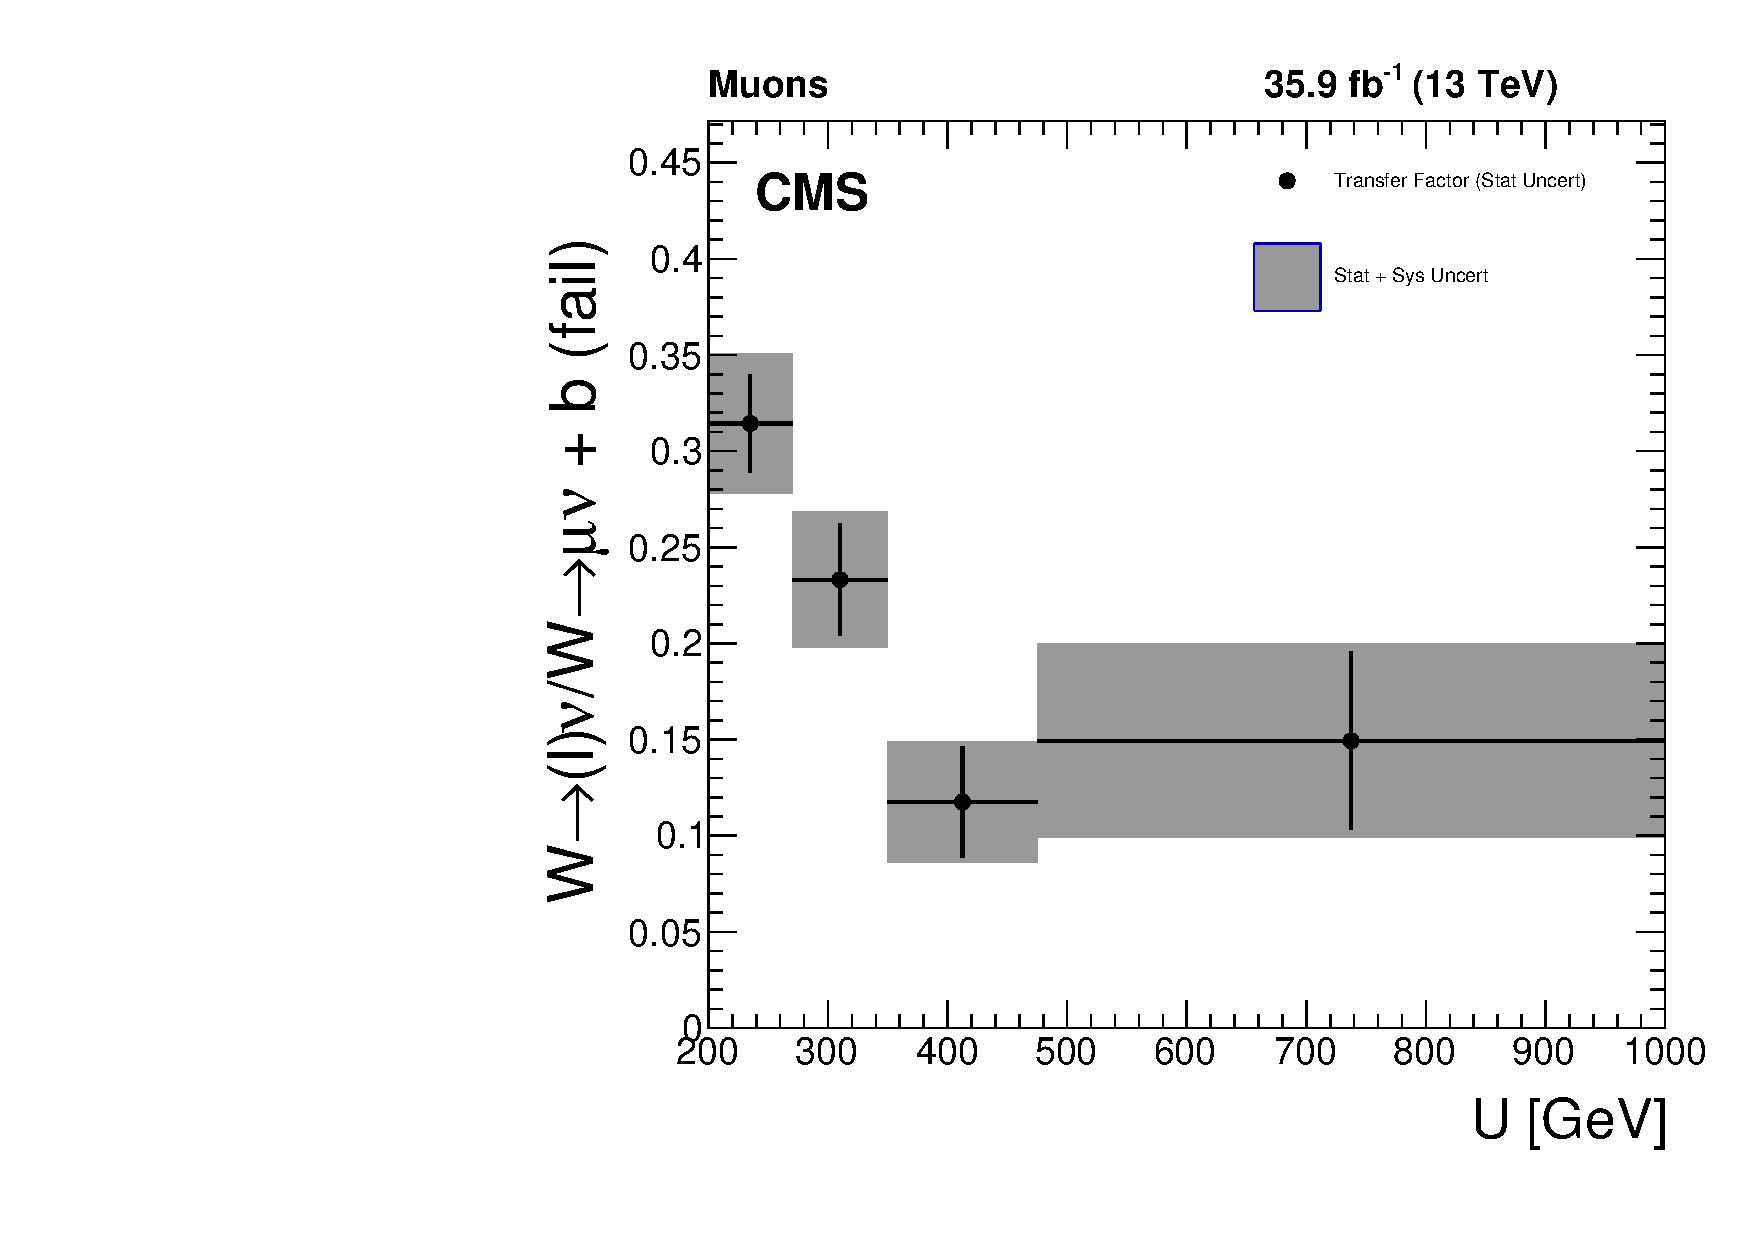
\includegraphics[width=0.25\textwidth]{figures/limits/rfactor_singlemuontopw_fail.pdf}
    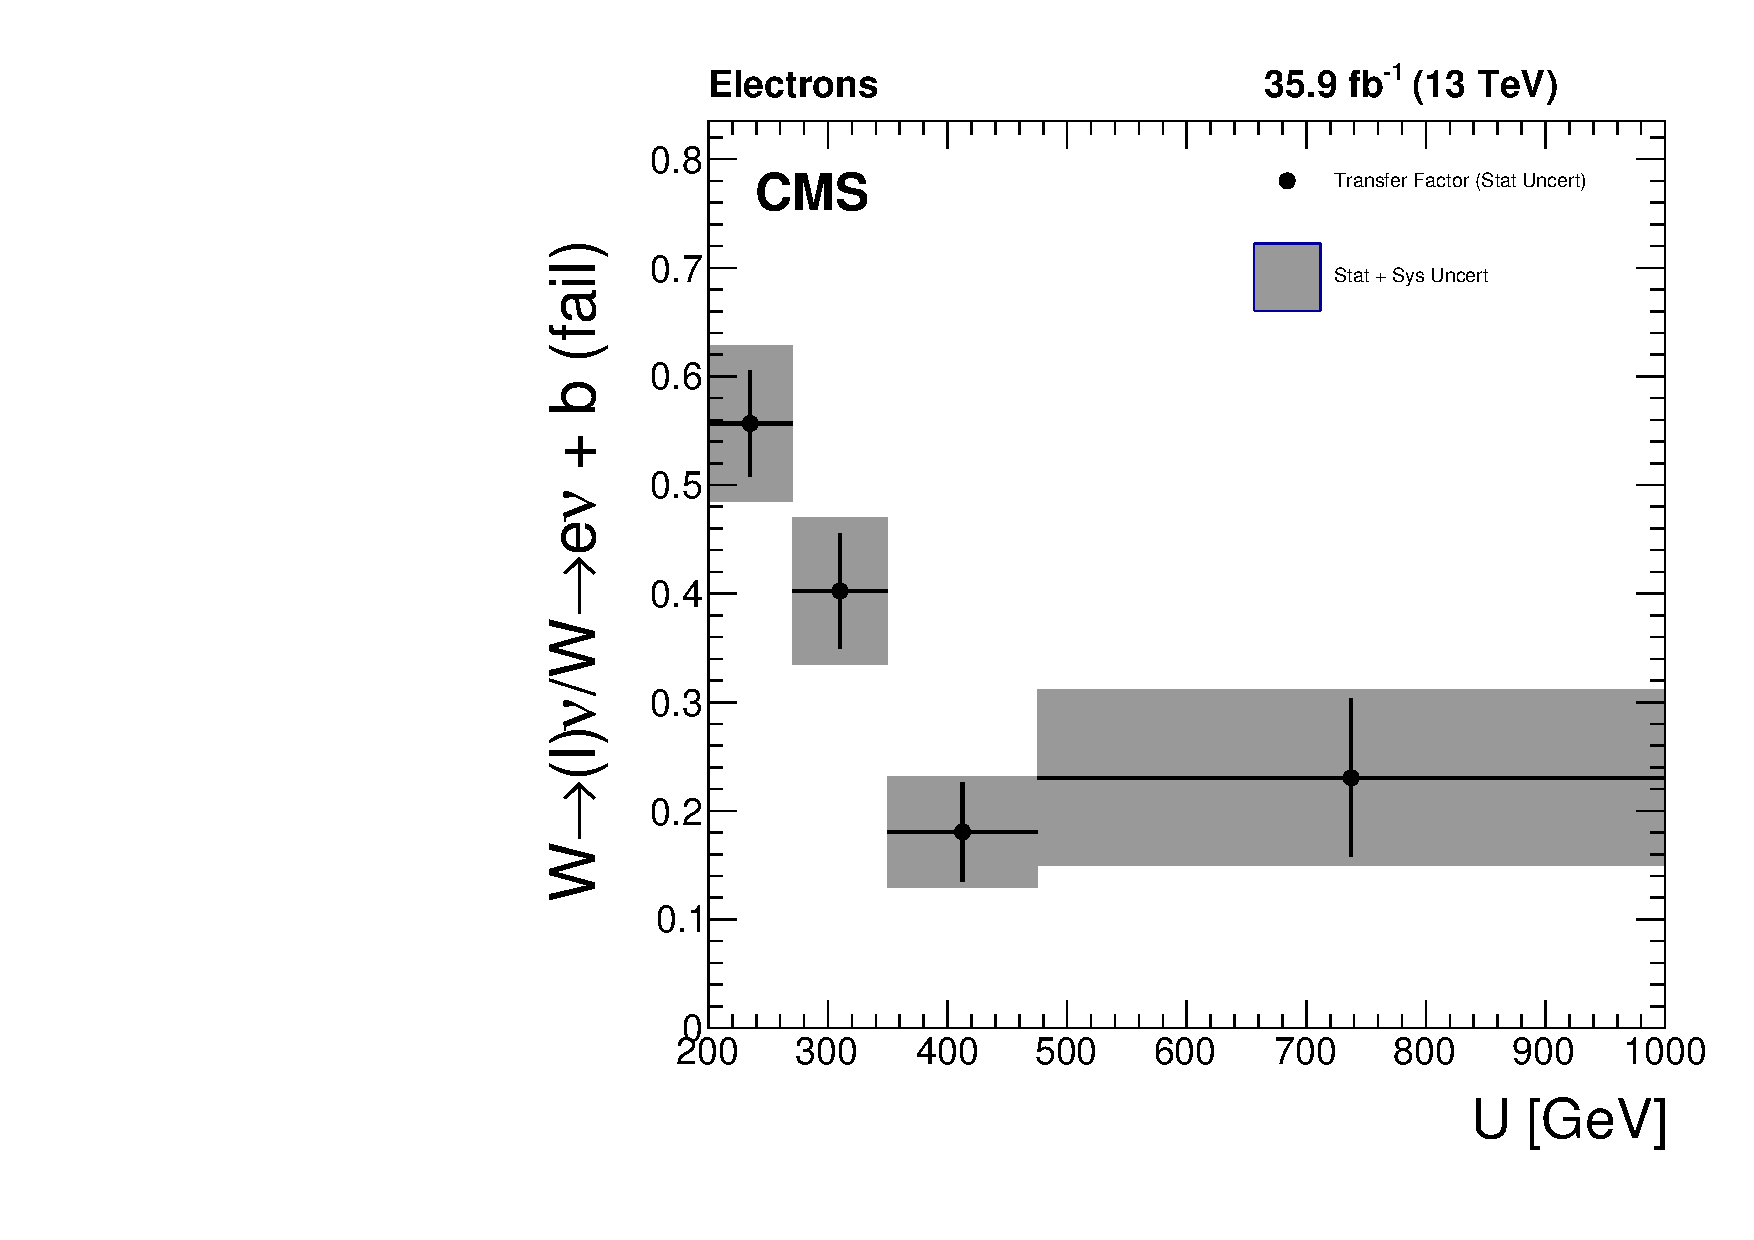
\includegraphics[width=0.25\textwidth]{figures/limits/rfactor_singleelectrontopw_fail.pdf}
  }\\
  \caption{Transfer factors to estimate $W$+jets in the signal region}
  \label{fig:xferW}
\end{figure}

%In order to validate the accuracy of the MC/MC transfer factors, we compare analogous transfer factors in the control regions.
%For example, to validate $(W\rightarrow(\ell)\nu)/(Z\rightarrow\nu\nu)$, we can look at $(W\rightarrow\mu\nu)/(Z\rightarrow\mu\mu)$ in both data and MC.
%Because the top-tag enhances top backgrounds in the control regions, the $t\bar{t}$ prediction (as well as other minor backgrounds) is subtracted from the data before building the data/data ratios.
%Similarly, the QCD prediction in the $\gamma$+jets CR is subtracted from the data.
%Figures~\ref{fig:rValidationLoose}-\ref{fig:rValidationTight} show this validation, including comparing $W/W$ and $Z/Z$ ratios between electrons and muons. 

%In general, the agreement is reasonable, except for ratios that involve the tight $Z\rightarrow\mu\mu$ control region.
%This can be observed in Figure~\ref{fig:rValidationTight} (top right, middle right, bottom left).
%This disagreement is due to the pre-fit discrepancy observed at high $U$ in Figure~\ref{fig:tightzmm}.
%In order to estimate the impact of this discrepancy on the robustness of the fit, a saturated goodness-of-fit test is performed.
%The test is performed only in the tight category to isolate this effect.
%The $-2\Delta\lambda$ of the GOF test on data is compared to 5000 toy datasets thrown from the MC prediction
%The distribution of the toys and the data value is shown in Figure~\ref{fig:goftight}.
%A $p$-value of $0.86$ indicates that the fit results are reasonable, despite the disagreement in these bins.





